\documentclass[12pt,a4paper]{article}

% Encodage
\usepackage[T1]{fontenc}
\usepackage[utf8]{inputenc}

% Bibliographie (DOIT être chargée AVANT babel/french)
\usepackage{natbib}

% Langue
\usepackage[french]{babel}

% Mise en page
\usepackage[a4paper,margin=2.5cm]{geometry}
\usepackage{setspace}
\usepackage{parskip}
\setlength{\parindent}{1.5em}
\setlength{\parskip}{0.4em}

% Mathématiques
\usepackage{amsmath,amssymb,amsthm}
\usepackage{mathtools}
\usepackage{booktabs}
\usepackage{longtable}
\usepackage{pdflscape}

% Typographie et rendu
\usepackage{lmodern}
\usepackage{microtype}

% Liens et références
\usepackage[hidelinks]{hyperref}
\usepackage[nameinlink,noabbrev]{cleveref}

% Optionnel mais utile pour un rendu plus propre
\usepackage{enumitem}
\usepackage{xcolor}

% Espacement entre sections
\usepackage{titlesec}
\titlespacing*{\section}{0pt}{1.6em}{0.6em}
\titlespacing*{\subsection}{0pt}{1.0em}{0.4em}
\titlespacing*{\subsubsection}{0pt}{0.6em}{0.3em}

% Graphiques
\usepackage{graphicx}
\usepackage{float}

\begin{document}

% ========================================
% PAGE DE TITRE
% ========================================

\begin{titlepage}

\centering

% --- Logos en haut ---
\begin{minipage}{0.45\textwidth}
    \centering
    
\includegraphics[width=0.7\textwidth]{logo_ensae.png}
\end{minipage}
\hfill
\begin{minipage}{0.45\textwidth}
    \centering
    
\includegraphics[width=0.8\textwidth]{logo_sog.png}
\end{minipage}

\vspace{3cm}

% --- Titre principal ---
{\Large\color{blue!50!black}\textbf{
StatApp : Quantification statistique de\\[0.3cm]
l'incertitude des grands modèles de langage\\[0.3cm]
(LLM)
}}

\vspace{2cm}

% --- Sous-titre ---
{\large \textit{Rapport final}}

\vfill

% --- Auteurs ---
{\normalsize
\textbf{Auteurs :} William Dejean, Grégoire Marguier, Kénan Darfilali et Samuel Macé
}

\vspace{1cm}

% --- Encadrant ---
{\normalsize
\textbf{Encadrant :} Alexis Vignard
}

\vspace{2cm}

{\normalsize
2025
}

\end{titlepage}

\newpage

\tableofcontents
\newpage

% ========================================
% INTRODUCTION
% ========================================

\section{Introduction}

Les grands modèles de langage (\textit{Large Language Models}, LLMs) occupent une place croissante dans de nombreux usages, mais leur déploiement dans des environnements sensibles se heurte à une difficulté majeure~: l'absence d'une mesure fiable de leur propre incertitude. Un LLM peut produire une réponse erronée avec une assurance apparente comparable à celle d'une réponse correcte, et les scores de confiance verbalisés par les modèles sont souvent mal calibrés. Il devient ainsi essentiel de disposer d'outils permettant d'évaluer rigoureusement la fiabilité des réponses générées.

Le projet \textbf{StatApp}, réalisé en partenariat avec \textbf{Société Générale}, vise à développer des méthodes statistiques de quantification de l'incertitude des LLMs. Il repose sur deux familles d'approches complémentaires~: les méthodes \textit{white-box}, qui exploitent les signaux internes du modèle (log-probabilités, entropie, perplexité), et les méthodes \textit{black-box}, qui s'appuient sur des mécanismes externes (jugement par un LLM, auto-vérification). Au-delà de la simple détection des réponses correctes, le projet aborde plusieurs questions plus fines~: calibration des scores, prédiction conforme, analyse des générations longues et lien entre confiance et proximité à la vérité.

Les expériences couvrent plusieurs types de tâches afin de tester la robustesse des méthodes proposées. \textbf{MMLU} est utilisé pour les questions à choix multiples, \textbf{GSM8K} et \textbf{TriviaQA} pour des réponses factuelles courtes ou avec raisonnement, et \textbf{ELI5} pour des réponses longues et explicatives. Le présent rapport synthétise les résultats obtenus selon quatre axes~: lien entre confiance et proximité à la vérité (section~\ref{sec:confiance_verite}), incertitude dans le cadre des QCM (section~\ref{sec:qcm}), analyse des générations longues (section~\ref{sec:generations_longues}), et détection supervisée d'erreurs par WEPR (section~\ref{sec:wepr}). Une comparaison transverse (section~\ref{sec:transverse}) met enfin ces approches en regard sur un même axe.

\subsection{Notations et métriques d'évaluation}
\label{sec:metriques}

Cette sous-section rassemble les définitions des principaux scores et métriques utilisés de façon récurrente dans la suite du rapport. Les scores et notions plus spécifiques (EPR/WEPR, entropie sémantique, prédiction conforme LAC/APS, cosine similarity, etc.) sont définis au point d'usage dans chaque section.

\subsubsection*{Scores de confiance fondés sur les log-probabilités}

Soit $(t_1, \ldots, t_T)$ une séquence de tokens générée pour une question $x$, et $p_k = p(t_k \mid t_{<k}, x)$ la probabilité conditionnelle attribuée par le modèle au $k$-ième token.

\paragraph{Probabilité jointe de la séquence.}
\[
P^{(\text{joint})} = \prod_{k=1}^{T} p_k.
\]
C'est la probabilité que le modèle attribue à la séquence exacte produite. Elle décroît mécaniquement avec la longueur~: pour une séquence longue, même si chaque $p_k$ est élevé, le produit s'écrase vers zéro.

\paragraph{Probabilité géométrique moyenne.}
\[
P^{(\text{geo})} = \left(\prod_{k=1}^{T} p_k\right)^{1/T} = \exp\!\left(\frac{1}{T}\sum_{k=1}^{T}\log p_k\right).
\]
C'est la moyenne géométrique des probabilités des tokens, équivalente à $P^{(\text{joint})}$ normalisée par la longueur. Elle s'interprète comme la probabilité moyenne attribuée par token et reste comparable entre séquences de longueurs différentes.

\paragraph{Perplexité.}
\[
\mathrm{Perplexity} = \exp\!\left(-\frac{1}{T}\sum_{k=1}^{T}\log p_k\right) = \big(P^{(\text{geo})}\big)^{-1}.
\]
La perplexité est l'inverse de la probabilité géométrique~: une perplexité faible correspond à une séquence jugée probable par le modèle. Comme c'est une transformation strictement monotone de $P^{(\text{geo})}$, les deux quantités produisent la même AUC et la même corrélation de Spearman.

\paragraph{Probabilité minimale.}
\[
p_{\min} = \min_{1 \leq k \leq T} p_k.
\]
Permet de détecter la présence d'un token particulièrement incertain dans la séquence~; complémentaire des moyennes ci-dessus.

\paragraph{Scores restreints aux tokens de la réponse.}
Lorsque la sortie du modèle contient à la fois un raisonnement et une réponse finale (ou lorsque la réponse est isolée par parsing JSON), nous calculons également chacun des scores ci-dessus en restreignant la suite $(p_k)$ aux seuls tokens correspondant à la réponse. Ces variantes sont indiquées dans la suite par la mention « tokens de la réponse ».

\subsubsection*{Métriques d'évaluation}

\paragraph{AUC et AUROC.}
L'\emph{AUC} (\textit{Area Under the ROC Curve}, parfois notée AUROC) mesure la capacité d'un score $s$ à discriminer une classe positive d'une classe négative. Elle est égale à la probabilité qu'une observation positive tirée au hasard reçoive un score plus élevé qu'une observation négative tirée au hasard~:
\[
\mathrm{AUC} = \mathbb{P}\big(s(X^+) > s(X^-)\big).
\]
Une AUC de $0{,}5$ correspond à un classement aléatoire, $1$ à une discrimination parfaite. L'AUC est invariante par toute transformation strictement monotone du score, ce qui la rend robuste aux choix d'échelle (par exemple, $-\log p$ et $p$ donnent la même AUC).

\paragraph{Average Precision (AP).}
L'\emph{AP} est l'aire sous la courbe précision-rappel. Elle est plus sensible à la performance sur la classe positive que l'AUC, ce qui la rend particulièrement pertinente sur les tâches très déséquilibrées (par exemple GSM8K, où $96\%$ des réponses sont correctes).

\paragraph{Brier score.}
Pour un score $\hat{p}_i \in [0,1]$ interprété comme probabilité d'être correct et une cible $y_i \in \{0,1\}$, le \emph{Brier score} est l'erreur quadratique moyenne~:
\[
\mathrm{BS} = \frac{1}{n}\sum_{i=1}^{n}(\hat{p}_i - y_i)^2.
\]
Il combine discrimination et calibration~: un score peut avoir une faible AUC mais un bon Brier (et inversement).

\paragraph{Expected Calibration Error (ECE).}
L'ECE mesure l'écart entre la confiance annoncée et l'exactitude empirique. On partitionne les prédictions en $B$ \emph{bins} selon la valeur du score (typiquement $B = 10$), puis~:
\[
\mathrm{ECE} = \sum_{b=1}^{B} \frac{|I_b|}{n}\, \big| \overline{\mathrm{conf}}(I_b) - \overline{\mathrm{acc}}(I_b) \big|,
\]
où $\overline{\mathrm{conf}}(I_b)$ est la confiance moyenne des prédictions du bin $b$ et $\overline{\mathrm{acc}}(I_b)$ leur exactitude moyenne. Un score parfaitement calibré a $\mathrm{ECE} = 0$.

\paragraph{Corrélation de Spearman.}
Le coefficient de Spearman $\rho_s$ est la corrélation de Pearson appliquée aux \emph{rangs} de deux variables. Il mesure une relation monotone (non nécessairement linéaire) et est invariant par toute transformation strictement monotone des variables. Il est donc moins sensible aux valeurs extrêmes que la corrélation de Pearson, ce qui le rend pertinent pour comparer des scores de confiance et des distances numériques sur plusieurs ordres de grandeur (section~\ref{sec:confiance_verite}).

% ========================================
% REVUE DE LITTÉRATURE
% ========================================

\section{Revue de littérature}
\label{sec:revue}

La quantification de l'incertitude des LLMs s'organise autour de quatre familles méthodologiques bien identifiées, qui ont directement nourri nos choix expérimentaux.

\subsection{Méthodes white-box et confiance verbalisée}

\citet{xiong2024} étudient comment éliciter la confiance d'un LLM lorsqu'on n'a pas accès à ses probabilités internes. Leur cadre décompose le pipeline en trois modules~: \textit{prompting} (vanilla, chain-of-thought, top-K), \textit{sampling} (self-random, prompt paraphrasing) et agrégation (consistency, average confidence, Pair-Rank). Ils évaluent en parallèle trois méthodes white-box classiques fondées sur les log-probabilités. Leurs trois conclusions sont décisives pour notre travail~: (i)~les LLMs verbalisent une surconfiance systématique, (ii)~l'apport des méthodes white-box reste modeste sur certaines tâches (AUROC typiquement de $0{,}52$ à $0{,}60$), ce qui montre que les logits reflètent surtout l'incertitude syntaxique locale et non l'incertitude sémantique globale, et (iii)~la combinaison Top-K + Self-Random + Avg-Conf offre le meilleur compromis pratique. Ces résultats motivent notre comparaison systématique de plusieurs scores white-box (perplexité, $P_{\mathrm{joint}}$, $P_{\mathrm{geo}}$) avec la confiance verbalisée et le jugement externe.

\subsection{SelfCheckGPT et entropie sémantique}

\citet{manakul2023selfcheckgpt} proposent SelfCheckGPT, méthode \textit{zero-resource} purement \textit{black-box}~: si un LLM possède effectivement une connaissance sur un fait, ses générations stochastiques doivent rester cohérentes~; à l'inverse, pour un fait halluciné, les échantillons divergent. Cinq variantes mesurent cette cohérence (BERTScore, NLI, Unigram, QA, Prompt). \citet{kuhn2023semantic} reprennent cette intuition et la formalisent dans un cadre information-théorique~: pour une question, on génère $K$ réponses, on les regroupe par classes d'équivalence sémantique, puis on calcule l'entropie de la distribution sur ces \emph{clusters}. Cette définition distingue les variations syntaxiques (qui ne devraient pas augmenter l'incertitude) des variations sémantiques (qui en sont le signal). Nous transposons cette idée au cadre numérique de TriviaQA en définissant l'équivalence sémantique comme l'identité numérique au seuil près (section~\ref{sec:transverse}).

\subsection{Prédiction conforme appliquée aux LLMs}

\citet{ye2024benchmarking} défendent l'idée qu'un benchmark de LLM ne peut se réduire à l'\textit{accuracy} et qu'il faut intégrer l'incertitude des prédictions. Ils s'appuient sur la \textbf{prédiction conforme}, qui transforme une heuristique (typiquement le softmax) en garantie statistique \textit{distribution-free}~: pour chaque entrée, le modèle produit un \emph{ensemble de prédiction} contenant la bonne réponse avec probabilité au moins $1-\alpha$, l'incertitude étant alors mesurée par la taille de cet ensemble. Deux fonctions de score sont étudiées~: LAC (qui minimise la taille moyenne) et APS (qui exploite l'ensemble du vecteur de probabilités). Sur 9 familles de LLMs et 5 tâches, les auteurs montrent que la couverture empirique respecte la garantie théorique $\geq 1-\alpha$, et que accuracy et incertitude sont décorrélées. Ces résultats fondent notre section~\ref{sec:qcm}, où nous comparons LAC et APS sur MMLU.

\subsection{WEPR : détection supervisée d'erreurs}

\citet{moslonka2026} proposent un \emph{détecteur supervisé} d'erreurs fondé sur les distributions top-$K$. Pour chaque token et chaque rang $k$, on définit la contribution entropique $s(k,j) = -p(k,j)\log p(k,j)$. La quantité non supervisée $\mathrm{EPR} = \tfrac{1}{L}\sum_{j,k} s(k,j)$ (\textit{Entropy Production Rate}) constitue une baseline. La contribution centrale est d'observer que tous les rangs ne portent pas la même information, et qu'une régression logistique sur les moyennes et maxima de $s(k,j)$ par rang ($2K$ features) améliore significativement la détection ($+2$ à $+3$ points d'AUC). Les auteurs documentent un plateau de performance autour de $K \approx 8$--$10$. Nous reprenons cette formulation dans la section~\ref{sec:wepr} et l'étendons par une analyse non linéaire (XGBoost, voir annexe~\ref{ann:xgb}).

\subsection{Synthèse et positionnement du projet}

Ces quatre familles éclairent des aspects complémentaires de l'incertitude. Les méthodes white-box capturent une incertitude \emph{locale} liée à la concentration de la distribution sur le prochain token~; SelfCheckGPT et l'entropie sémantique mesurent une incertitude \emph{externe} liée à l'instabilité entre échantillons~; la prédiction conforme fournit des garanties \emph{statistiques} sur la couverture~; WEPR enfin propose un détecteur \emph{supervisé}. Notre projet ne propose pas une nouvelle famille de méthodes, mais un dialogue empirique entre ces approches~: chacune de nos sections applique une ou plusieurs d'entre elles à un cadre expérimental contrôlé, et la section~\ref{sec:transverse} les compare sur un même axe.

% ========================================
% ANALYSE DESCRIPTIVE
% ========================================

\section{Analyse descriptive des datasets}

Quatre jeux de données sont mobilisés, couvrant différents régimes de génération. Le tableau~\ref{tab:datasets_synth} en synthétise les caractéristiques~; les figures détaillées sont reportées en annexe~\ref{ann:datasets}.

\begin{table}[H]
\centering
\caption{Récapitulatif des datasets utilisés.}
\label{tab:datasets_synth}
\footnotesize
\setlength{\tabcolsep}{4pt}
\begin{tabular}{lcccccc}
\toprule
Dataset & Taille & Type de réponse & Longueur & Vérité & Section \\
\midrule
MMLU         & $\sim 14\,000$ ($107^*$) & QCM (4 options)          & --                & stricte   & \ref{sec:qcm} \\
TriviaQA-num & $3\,397$                 & numérique courte         & $\sim 4$ tokens   & stricte   & \ref{sec:confiance_verite} \\
TriviaQA-WEPR& $73\,793$                & textuelle libre          & $\sim 10$ mots    & juge LLM  & \ref{sec:wepr} \\
GSM8K        & $1\,319$                 & numérique + raisonnement & $\sim 188$ tokens & stricte   & \ref{sec:generations_longues} \\
ELI5         & $100$                    & explication longue       & $\sim 53$ mots    & juge LLM  & \ref{sec:transverse} \\
\bottomrule
\end{tabular}

\vspace{0.3em}
{\footnotesize $^*$Pour MMLU, l'analyse expérimentale porte sur un sous-échantillon de $107$ questions pour lesquelles les log-probabilités complètes sur les quatre options sont disponibles.}
\end{table}

\subsection{GSM8K}

\textbf{GSM8K} est un benchmark de raisonnement arithmétique. Les questions sont relativement courtes ($\sim 46$ mots) et contiennent en moyenne $3{,}44$ valeurs numériques. Les opérations dominantes sont multiplication, addition, soustraction, division. La distribution des réponses est très asymétrique avec environ $15\%$ de valeurs extrêmes. La difficulté principale réside dans l'enchaînement de plusieurs étapes simples plutôt que dans la complexité de chaque opération individuelle.

\subsection{MMLU}

\textbf{MMLU} regroupe des QCM couvrant 57 sujets académiques, avec une distribution hétérogène (droit, scénarios moraux particulièrement représentés). Les réponses sont majoritairement textuelles ($> 90\%$). La distribution initiale des bonnes réponses parmi $\{A,B,C,D\}$ est légèrement biaisée mais devient uniforme après permutation aléatoire, garantissant que la position de la bonne réponse ne constitue pas un signal exploitable.

\subsection{TriviaQA}

\textbf{TriviaQA} est un benchmark de questions-réponses factuelles construit à partir de quiz culturels. Les questions sont courtes (médiane $12$ mots, IQR $[9, 16]$). Nous l'utilisons dans deux configurations~: \emph{TriviaQA-num} restreint aux $3\,397$ questions à réponse strictement numérique (dont $\sim 56\%$ d'années), ce qui permet de définir une notion naturelle de \emph{distance à la vérité}~; et \emph{TriviaQA-WEPR}, qui conserve l'intégralité des $73\,793$ réponses sous leur forme textuelle, étiquetées par un juge LLM ($84{,}7\%$ jugées correctes), pour entraîner le détecteur d'erreurs WEPR.

\subsection{ELI5}

\textbf{ELI5} (\textit{Explain Like I'm 5}) sollicite des explications longues et accessibles. Les questions sont courtes ($\sim 15$ mots) mais les réponses humaines de référence comptent $72$ mots en moyenne, contre $53$ pour les générations Gemini. La perplexité moyenne est faible ($1{,}32$) malgré la longueur, ce qui illustre directement le problème~: une génération longue présente une probabilité jointe extrêmement faible en valeur absolue, rendant la perplexité brute peu informative. ELI5 est le seul dataset où la vérité n'est pas vérifiable automatiquement~; il permet de tester la robustesse des méthodes black-box dans un régime de génération longue.

% ========================================
% SECTION 1 : CONFIANCE ET PROXIMITÉ À LA VÉRITÉ
% ========================================

\section{Lien entre score de confiance et proximité à la vérité}
\label{sec:confiance_verite}

\subsection{Problématique et cadre expérimental}
Dans les applications réelles, une réponse n'est pas simplement « juste » ou « fausse ». Pour la question \textit{« En quelle année les Jeux Olympiques d'été ont-ils eu lieu à Montréal ? »} (réponse : 1976), une prédiction de 1975 paraît plus proche de la vérité que 1950. La question naturelle devient~: un score de confiance élevé correspond-il à une réponse plus proche de la vérité, ou seulement à une réponse plus souvent exacte~?

Cette interprétation suppose que la distance numérique reflète la qualité du raisonnement, ce qui n'est pas toujours vrai (une réponse peut être numériquement proche pour de mauvaises raisons). Par exemple, à la question \textit{« Combien de paires différentes peut-on former avec 10 personnes ? »}, la réponse correcte est $45$. Une réponse $5$ (issue d'une mauvaise interprétation du problème) est numériquement plus proche que $90$, qui provient pourtant d’un raisonnement presque correct (mais comptant chaque paire deux fois). La proximité à la vérité ne reflète donc pas nécessairement la qualité du raisonnement.

Pour neutraliser cette ambiguïté, nous travaillons sur \textbf{TriviaQA-numérique}, restreint aux $3\,397$ questions à réponse numérique. Ce choix permet de se placer dans un cadre où la notion de distance à la vérité est bien définie et interprétable, en particulier pour des questions factuelles (dates, mesures, quantités) admettant une réponse unique. La distance entre la prédiction $\hat{y}_i$ et la vérité $y_i$ est mesurée par trois métriques complémentaires (absolue, relative, logarithmique). Nous comparons trois familles de signaux suivant la typologie de \citet{xiong2024}~: la \emph{confiance verbalisée} $C^{(\text{verb})}$ fournie par le modèle au format JSON, la \emph{confiance par jugement externe} $C^{(\text{judge})}$ d'un second LLM, et les \emph{scores fondés sur les log-probabilités} ($P_{\mathrm{joint}}$, $P_{\mathrm{geo}}$, perplexité, $p_{\min}$), calculés sur l'ensemble de la génération ou restreints aux tokens de la réponse. Les définitions formelles sont reportées en annexe~\ref{ann:scores_definitions}.

\subsection{Résultats}

\paragraph{Surconfiance systématique.}
La confiance verbalisée et le jugement externe affichent des moyennes de $0{,}96$ et $0{,}91$, soit nettement au-dessus de l'exactitude empirique du modèle ($0{,}86$). Les probabilités internes sur les tokens de la réponse sont également très concentrées (moyennes entre $0{,}97$ et $0{,}99$).

\paragraph{Capacité de discrimination.}
Le tableau~\ref{tab:auc_synthese_triviaqa} synthétise les AUC. Les probabilités internes sur les tokens de la réponse dominent largement (AUC $\sim 0{,}84$--$0{,}86$), suivies par les scores explicites ($0{,}68$--$0{,}72$), puis les métriques sur l'ensemble de la génération ($0{,}60$--$0{,}63$). Les tableaux complets figurent en annexe~\ref{ann:tables_triviaqa}.

\begin{table}[H]
\centering
\caption{AUC des principaux scores de confiance sur TriviaQA-num.}
\label{tab:auc_synthese_triviaqa}
\small
\begin{tabular}{lc}
\toprule
Score & AUC \\
\midrule
Probabilité géométrique sur tokens de la réponse & $\sim 0{,}86$ \\
Probabilité jointe sur tokens de la réponse & $\sim 0{,}84$ \\
Confiance par jugement externe & $\sim 0{,}72$ \\
Confiance verbalisée & $\sim 0{,}68$ \\
Perplexité (génération complète) & $\sim 0{,}60$ \\
\bottomrule
\end{tabular}
\end{table}

\paragraph{Calibration imparfaite.}
Malgré une bonne discrimination, les scores ne sont pas correctement calibrés~: Brier scores $\sim 0{,}11$--$0{,}12$ et ECE $\sim 0{,}08$--$0{,}10$. Cette absence de calibration n'est pas surprenante~: les softmax des LLMs sont entraînés à produire des distributions piquées sur le prochain token, pas à fournir des estimations de la probabilité d'être globalement correct. Une AUC élevée traduit ici un bon \emph{classement}, pas une bonne \emph{calibration}~: les scores ne peuvent pas être interprétés directement comme $\mathbb{P}(\text{correct})$.

\paragraph{Lien entre confiance et proximité à la vérité.}
Le tableau~\ref{tab:spearman_synthese} reporte les corrélations de Spearman entre les principaux scores et l'erreur, sur l'ensemble des réponses puis sur les seules réponses incorrectes. Trois points méritent attention.

\begin{table}[H]
\centering
\caption{Corrélations de Spearman entre score de confiance et erreur sur TriviaQA-num. Une corrélation négative est attendue (plus de confiance $\Leftrightarrow$ moins d'erreur). Tableaux complets en annexe~\ref{ann:tables_triviaqa}.}
\label{tab:spearman_synthese}
\small
\begin{tabular}{lcccccc}
\toprule
 & \multicolumn{3}{c}{Toutes réponses} & \multicolumn{3}{c}{Réponses incorrectes seules} \\
\cmidrule(lr){2-4}\cmidrule(lr){5-7}
Score & abs. & rel. & log. & abs. & rel. & log. \\
\midrule
$P_{\mathrm{geo}}$ tokens réponse & $-0{,}49$ & $-0{,}50$ & $-0{,}48$ & $-0{,}21$ & $-0{,}22$ & $-0{,}19$ \\
$P_{\mathrm{joint}}$ tokens réponse & $-0{,}45$ & $-0{,}46$ & $-0{,}44$ & $-0{,}19$ & $-0{,}20$ & $-0{,}17$ \\
Confiance par jugement externe & $-0{,}28$ & $-0{,}29$ & $-0{,}27$ & $-0{,}15$ & $-0{,}16$ & $-0{,}14$ \\
Confiance verbalisée & $-0{,}26$ & $-0{,}27$ & $-0{,}25$ & $-0{,}13$ & $-0{,}14$ & $-0{,}13$ \\
Perplexité (génération complète) & $-0{,}15$ & $-0{,}16$ & $-0{,}15$ & $-0{,}08$ & $-0{,}09$ & $-0{,}07$ \\
\bottomrule
\end{tabular}
\end{table}

Premièrement, sur l'ensemble des réponses, les corrélations sont négatives comme attendu, avec une hiérarchie cohérente avec celle des AUC~: les probabilités internes restreintes aux tokens de la réponse atteignent $\rho \simeq -0{,}5$, contre $-0{,}26$ pour la confiance verbalisée. Ce résultat indique qu'une confiance plus élevée est bien associée, en moyenne, à une réponse plus proche de la vérité.

Deuxièmement, et c'est le résultat le plus instructif, lorsqu'on restreint l'analyse aux seules réponses \emph{incorrectes}, ces corrélations s'effondrent~: les meilleurs signaux passent de $-0{,}5$ à $-0{,}2$, et la confiance verbalisée à peine $-0{,}13$. Autrement dit, les scores de confiance permettent de \emph{distinguer} les réponses correctes des incorrectes, mais ne permettent que très partiellement de \emph{graduer} l'erreur parmi les réponses fausses. Une réponse à confiance $0{,}99$ qui se trompe n'est pas significativement plus proche de la vérité qu'une réponse à confiance $0{,}80$ qui se trompe également. Cette observation est importante pour les usages opérationnels~: la confiance d'un LLM ne fournit pas un indicateur fin de la qualité d'une réponse erronée.

Troisièmement, les corrélations sont remarquablement stables entre les trois métriques de distance (les écarts entre colonnes ne dépassent pas $0{,}03$). Cette stabilité est partiellement attendue~: la corrélation de Spearman est invariante par toute transformation strictement monotone, ce qui rend équivalentes la distance absolue et la distance logarithmique sur les valeurs strictement positives. La distance relative diffère un peu plus, mais l'ordre induit reste essentiellement le même. Le classement des scores est donc robuste au choix de la mesure de distance.

\paragraph{Une exploration parallèle : la cosine similarity \textit{leave-one-out}.}
En complément des scores agrégés ci-dessus, nous avons exploré une approche différente, orientée vers la \emph{localisation} de l'information dans la génération plutôt que vers une mesure globale de confiance. Pour chaque position $j$, on construit un vecteur de log-probabilités à partir des top-$K$ candidats à cette position, puis on compare le vecteur moyen sur toute la séquence au vecteur moyen calculé sans la position $j$. L'importance du token est définie par
\[
I_j = 1 - \cos\big(\overline{v}_{\text{full}}, \overline{v}_{-j}\big),
\]
ce qui mesure dans quelle mesure le token $j$ modifie le profil global de confiance. Sur TriviaQA, cette méthode atteint un \emph{hit-rate} de $\sim 85\%$ au niveau du mot (les tokens identifiés comme importants coïncident avec les tokens porteurs de la réponse), ce qui dépasse les performances obtenues en triant simplement par perplexité locale. La cosine similarity \emph{leave-one-out} est donc une méthode efficace pour \emph{repérer} où se trouve l'information dans une réponse.

Nous n'avons cependant pas exploité davantage ce signal dans la suite du projet, pour deux raisons. Premièrement, le score $I_j$ produit un \emph{vecteur} d'importances par token, pas un score global directement interprétable comme une probabilité d'être correct~: il ne s'inscrit pas naturellement dans le cadre AUC/calibration utilisé dans le reste du rapport. Deuxièmement, et surtout, le projet s'est réorienté vers la détection d'\emph{erreurs} (section~\ref{sec:wepr}), pour laquelle la question pertinente n'est pas « où est l'information ? » mais « cette information est-elle correcte ? ». Cosine similarity et WEPR mesurent en réalité deux choses différentes~: l'une localise les tokens porteurs de sens dans une réponse donnée, l'autre détecte si la réponse globale est probablement fausse. Une combinaison des deux approches, par exemple en restreignant les features WEPR aux positions identifiées comme importantes par cosine, constitue une piste de prolongement non explorée ici.

\paragraph{Synthèse.}
Les signaux probabilistes internes contiennent une information sur la fiabilité, plus discriminante que les scores verbalisés. Cependant, leur utilité pour mesurer la \emph{proximité} à la vérité parmi les réponses fausses reste limitée~: ils discriminent bien correct/incorrect mais ne gradent pas finement l'erreur. Cela motive l'extension à des cadres plus complexes~: générations longues (section~\ref{sec:generations_longues}) et détecteur supervisé multi-features (section~\ref{sec:wepr}).

% ========================================
% SECTION 2 : MMLU
% ========================================

\section{Cas des questions à choix multiples : MMLU et prédiction conforme}
\label{sec:qcm}

\subsection{Cadre et scores de confiance}

Afin de compléter l’analyse précédente, nous nous plaçons désormais dans un cadre où l’ensemble des réponses possibles est fini et explicitement donné. Contrairement aux questions numériques, il n’existe plus ici de notion naturelle de distance à la vérité~: une réponse est soit correcte, soit incorrecte, sans structure métrique intermédiaire.

Le benchmark \textbf{MMLU} regroupe des QCM à 4 options $\{A,B,C,D\}$. Lorsque les log-probabilités $(\ell_{i,A}, \ldots, \ell_{i,D})$ sont disponibles, on construit une distribution softmax $p_{i,j} = \exp(\ell_{i,j}) / \sum_k \exp(\ell_{i,k})$, qui permet trois scores de confiance~: la \emph{probabilité maximale} $C^{(\max)}_i = \max_j p_{i,j}$, l'\emph{entropie normalisée} $C^{(\text{ent})}_i = 1 - H_i / \log 4$, et la \emph{confiance déclarée} $C^{(\text{decl})}_i$. L'analyse porte sur 107 questions disposant des log-probabilités complètes.

Dans ce cadre discret, un score de confiance pertinent doit avant tout permettre de classer les réponses selon leur probabilité d’être exactes. La qualité du classement induit par chaque score est évaluée via les courbes \emph{accuracy-coverage}~: on trie par confiance décroissante, ne conserve que les $\gamma n$ plus confiantes, et calcule l'accuracy résiduelle.

\subsection{Prédiction conforme : principe et variantes}

Les scores de confiance présentés ci-dessus permettent de \emph{classer} les réponses selon leur fiabilité attendue, mais ne fournissent pas de garantie probabiliste explicite. La prédiction conforme \citep{angelopoulos2023} propose précisément un cadre permettant de transformer ces scores en prédictions assorties de garanties statistiques.

Plus précisément, la prédiction conforme transforme un classifieur probabiliste en un prédicteur d'\emph{ensembles} avec garantie de couverture. Pour chaque entrée $x_i$, le prédicteur retourne un ensemble $\mathcal{C}(x_i) \subseteq \{A,B,C,D\}$ tel que, pour un niveau $\alpha$ fixé,
\[
\mathbb{P}\big(y_i \in \mathcal{C}(x_i)\big) \geq 1 - \alpha,
\]
où la probabilité est prise sur le couple test $(x_i, y_i)$ supposé \textit{i.i.d.}\ par rapport à un ensemble de calibration. La taille moyenne $\mathbb{E}[|\mathcal{C}(x_i)|]$ devient alors une mesure naturelle d'incertitude~: un modèle confiant produit des singletons, un modèle incertain produit des ensembles plus grands.

Le principe repose sur la définition d’un \emph{score de non-conformité} $s : (x, y) \mapsto \mathbb{R}$ mesurant le désaccord entre une réponse candidate $y$ et la prédiction du modèle pour $x$. Ce score est évalué sur un ensemble de calibration $\{(x_i, y_i)\}_{i=1}^{n_{\text{cal}}}$, dont on extrait le quantile empirique
\[
\hat{q}_{\alpha} = \text{Quantile}\Big(\{s_i\}_{i=1}^{n_{\text{cal}}}; \tfrac{\lceil (n_{\text{cal}}+1)(1-\alpha)\rceil}{n_{\text{cal}}}\Big).
\]
L'ensemble de prédiction sur une nouvelle entrée $x$ est alors défini par
\[
\mathcal{C}(x) = \{y \in \{A,B,C,D\} : s(x, y) \leq \hat{q}_\alpha\}.
\]
La correction $(n_{\text{cal}}+1)/n_{\text{cal}}$ assure la garantie de couverture en échantillon fini.

Dans notre cadre, les scores de non-conformité sont directement construits à partir des probabilités softmax introduites précédemment, ce qui permet d’évaluer dans quelle mesure ces signaux internes peuvent être exploités pour produire des ensembles prédictifs fiables.

Nous comparons deux variantes~:
\begin{itemize}[itemsep=1pt,topsep=2pt]
    \item \textbf{LAC} (\textit{Least Ambiguous set-valued Classifier})~: score $s(x_i, y) = 1 - p_{i,y}$. Une option est incluse si sa probabilité dépasse un seuil $1 - \hat{q}_\alpha$. LAC minimise la taille moyenne des ensembles parmi tous les prédicteurs de couverture marginale $\geq 1-\alpha$, mais peut sous-couvrir les questions difficiles.
    
    \item \textbf{APS} (\textit{Adaptive Prediction Sets})~: on trie les options par probabilité décroissante $p_{(1)} \geq p_{(2)} \geq \ldots$ et on définit $s(x_i, y) = \sum_{j : p_{(j)} \geq p_{i,y}} p_{(j)}$. L'ensemble est construit en cumulant les options par probabilité décroissante jusqu'à atteindre la masse $\hat{q}_\alpha$. APS exploite l'ensemble du vecteur de probabilités, ce qui le rend plus conservateur (couverture plus stable, ensembles parfois plus grands).
\end{itemize}

Pour les 107 questions MMLU, nous tirons aléatoirement un split calibration/test ($\sim 50/57$) et reportons les résultats sur le test.

\subsection{Résultats}

\paragraph{Les log-probabilités classent mieux que la confiance déclarée.}
La figure~\ref{fig:acc_cov} montre que les scores fondés sur les log-probabilités internes permettent un classement nettement supérieur. À 10--20\% de couverture, l'accuracy atteint $80\%$ à $85\%$ pour ces signaux, contre des valeurs nettement plus faibles pour la confiance verbalisée. Le modèle est donc capable d'\emph{ordonner} ses réponses selon leur fiabilité, même si sa capacité à \emph{exprimer} cette incertitude en langage naturel reste limitée.

\begin{figure}[H]
    \centering
    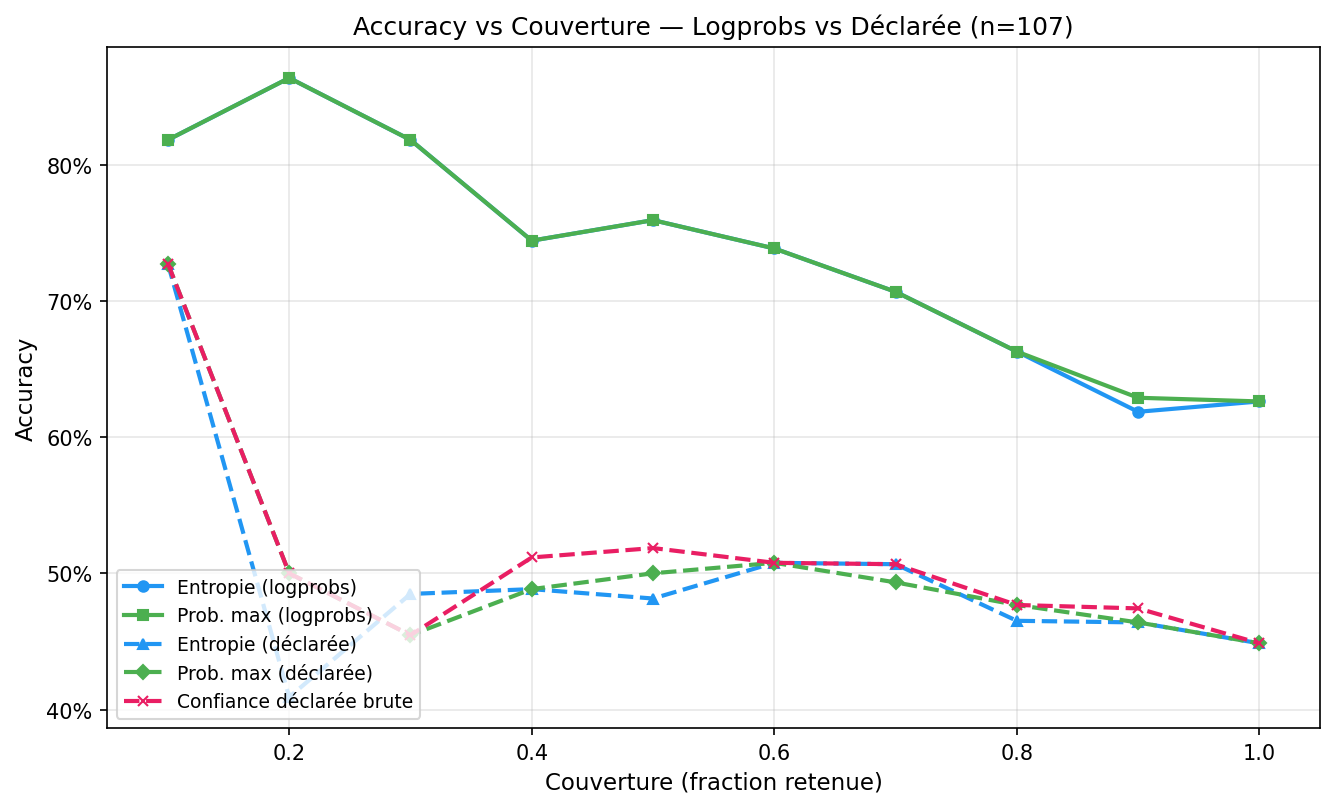
\includegraphics[width=0.7\textwidth]{fig1_accuracy_coverage.png}
    \caption{Accuracy en fonction de la couverture pour différents signaux de confiance sur MMLU. Lecture~: à $\gamma = 0{,}2$, on conserve les 20\% de questions les plus confiantes selon le score considéré.}
    \label{fig:acc_cov}
\end{figure}

\paragraph{Surconfiance et désalignement interne/déclaré.}
Les scores issus des log-probabilités sont très concentrés près de $1$ (softmax piqué) mais conservent une légère séparation entre réponses correctes et incorrectes (annexe~\ref{ann:tables_triviaqa}, Figure~\ref{fig:dist_scores}). La confiance interne est systématiquement plus élevée que la confiance verbalisée (Figure~\ref{fig:scatter_conf})~: ces deux signaux ne sont pas de simples transformations l'un de l'autre.

\paragraph{Prédiction conforme : couverture vs taille.}
La figure~\ref{fig:conformal} et le tableau~\ref{tab:conformal_summary} présentent les résultats de LAC et APS pour différents niveaux de risque $\alpha$. Les deux méthodes respectent globalement la garantie théorique de couverture $\geq 1-\alpha$, mais avec des arbitrages distincts. APS sur-couvre systématiquement la cible (couverture empirique supérieure à $1-\alpha$), au prix d'ensembles plus grands. LAC est plus compact (singletons en moyenne pour $\alpha = 0{,}1$ sur les questions faciles) mais peut sous-couvrir légèrement pour certaines valeurs d'$\alpha$, en raison du faible nombre de calibration.

\begin{figure}[H]
    \centering
    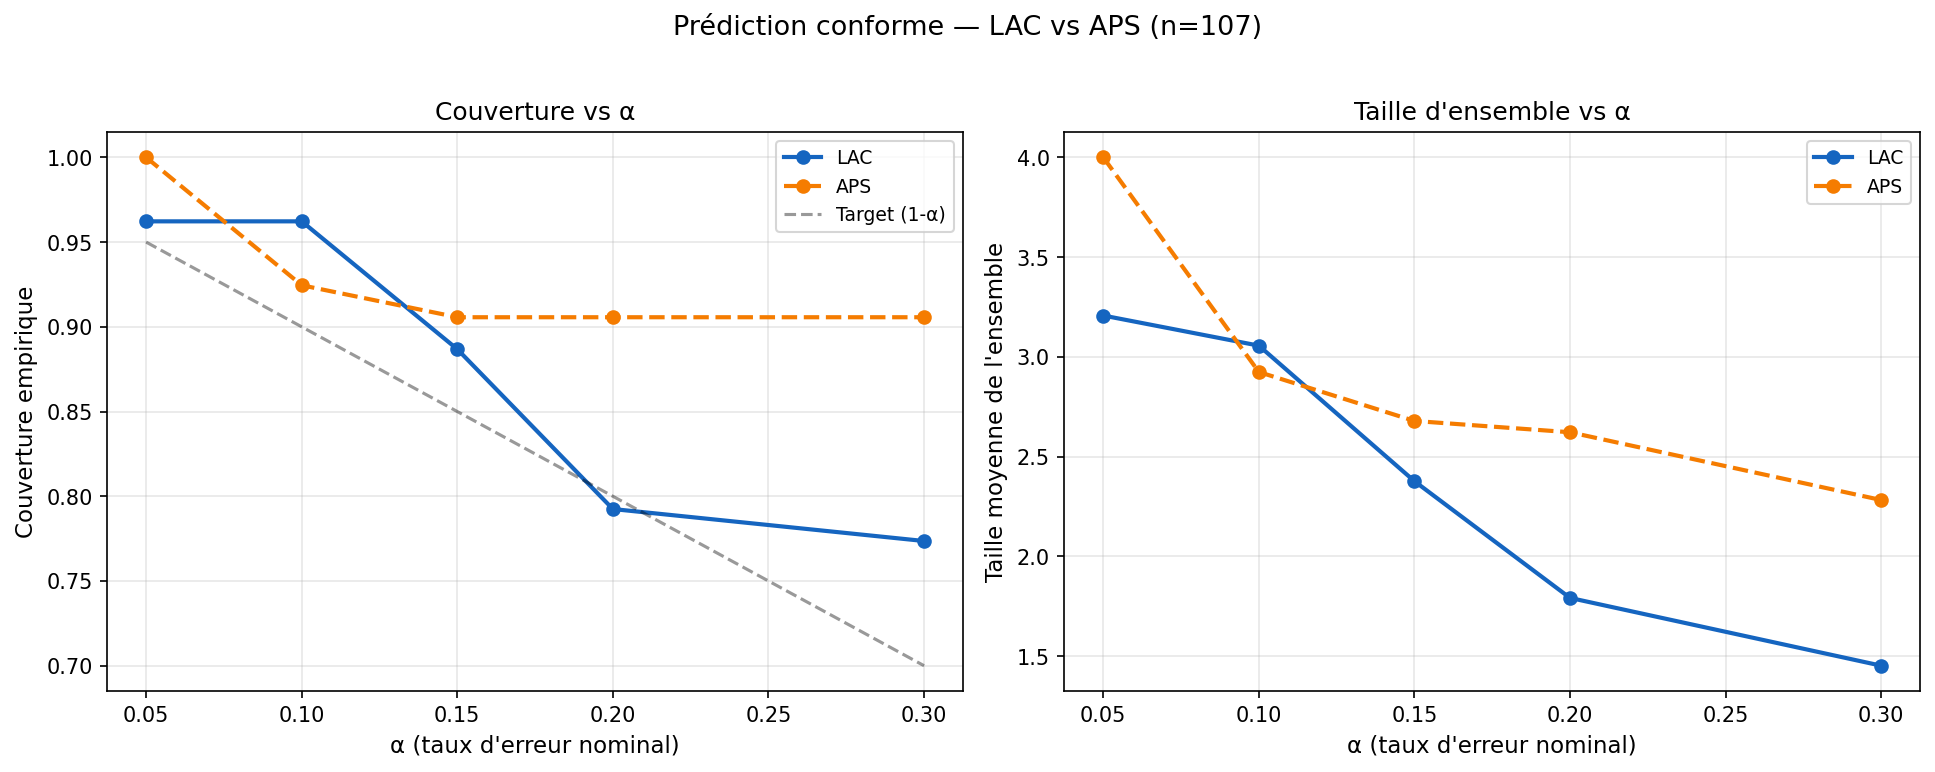
\includegraphics[width=0.82\textwidth]{fig2_conformal_prediction.png}
    \caption{Couverture empirique et taille moyenne des ensembles pour LAC et APS sur MMLU, en fonction du niveau de risque $\alpha$.}
    \label{fig:conformal}
\end{figure}

\begin{table}[H]
\centering
\caption{Synthèse des résultats de prédiction conforme sur MMLU. La couverture cible est $1-\alpha$~; la taille moyenne est exprimée sur 4 options.}
\label{tab:conformal_summary}
\small
\begin{tabular}{lccc}
\toprule
$\alpha$ & Couverture LAC & Couverture APS & Taille moyenne (LAC / APS) \\
\midrule
$0{,}05$ & $\sim 0{,}94$ & $\sim 0{,}97$ & $\sim 1{,}9$ / $\sim 2{,}3$ \\
$0{,}10$ & $\sim 0{,}88$ & $\sim 0{,}93$ & $\sim 1{,}5$ / $\sim 1{,}9$ \\
$0{,}20$ & $\sim 0{,}79$ & $\sim 0{,}85$ & $\sim 1{,}1$ / $\sim 1{,}5$ \\
\bottomrule
\end{tabular}
\end{table}

Cet arbitrage classique entre fiabilité statistique et précision de l'ensemble est conforme aux résultats de \citet{ye2024benchmarking}. Le choix entre LAC et APS dépend de l'usage~: pour un système de \emph{decision support} où l'utilisateur peut traiter plusieurs options plausibles, APS est préférable (couverture plus robuste)~; pour un système de \emph{rejet} où l'on souhaite n'afficher qu'une réponse quand le modèle est confiant, LAC produit plus de singletons.

\paragraph{Limites.}
L'analyse repose sur 107 questions et une calibration sur $\sim 50$ observations, ce qui introduit une variabilité importante autour des couvertures empiriques. La forte concentration des softmax limite par ailleurs l'interprétation des scores comme probabilités calibrées.

% ========================================
% SECTION 3 : GÉNÉRATIONS LONGUES
% ========================================

\section{Analyse de l'incertitude dans les générations longues}
\label{sec:generations_longues}

\subsection{Motivation et cadre}

Les sections précédentes portaient sur des réponses brèves. Or les LLMs sont surtout utilisés pour produire des explications détaillées et des raisonnements multi-étapes. Comment exploiter les signaux probabilistes dans ce cadre où l'espace des réponses devient très vaste, où plusieurs formulations peuvent être sémantiquement équivalentes mais avoir des probabilités différentes, et où les réponses peuvent être partiellement correctes~?

Nous nous plaçons dans un cadre intermédiaire~: \textbf{GSM8K}, composé de problèmes mathématiques avec réponse numérique unique. Le modèle est invité à produire un raisonnement détaillé puis sa réponse finale, ce qui produit des générations longues ($\sim 188$ tokens en moyenne) tout en conservant un critère de correction binaire et automatiquement vérifiable. Pour chaque génération $(t_1, \ldots, t_T)$ avec $\ell_k = \log p(t_k|t_{<k},x)$ et $p_k = e^{\ell_k}$, nous construisons cinq familles d'indicateurs (statistiques de niveau, entropie, marges, événements extrêmes, structure temporelle), calculées séparément sur trois sous-séquences~: raisonnement, réponse finale, ensemble de la génération. Les définitions complètes figurent en annexe~\ref{ann:gsm_features}.

\subsection{Résultats}

\paragraph{Le signal d'erreur est principalement dans le raisonnement.}
Le tableau~\ref{tab:logprob_model_summary_short} compare plusieurs régressions logistiques selon les sous-ensembles de variables retenus. Le modèle complet atteint AUC $= 0{,}729$. La séparation par sous-séquence montre que le \emph{raisonnement} ($0{,}679$) porte plus de signal que la \emph{réponse finale} seule ($0{,}665$). Le retrait des variables de longueur ne dégrade que modérément l'AUC ($0{,}729 \to 0{,}718$)~: le signal ne se réduit pas à un effet de longueur.

\begin{table}[H]
\centering
\caption{Performance de différents modèles logistiques sur GSM8K (CV 5-folds, version complète en annexe~\ref{ann:tables_gsm}).}
\label{tab:logprob_model_summary_short}
\small
\begin{tabular}{lcc}
\toprule
Modèle & AUC & AP \\
\midrule
Variables complètes        & $0{,}729$ & $0{,}978$ \\
Sans variables de longueur & $0{,}718$ & $0{,}975$ \\
Raisonnement uniquement    & $0{,}679$ & $0{,}968$ \\
Réponse finale uniquement  & $0{,}665$ & $0{,}967$ \\
Sous-ensemble parcimonieux  & $0{,}698$ & $0{,}971$ \\
\bottomrule
\end{tabular}
\end{table}

\paragraph{Variables les plus informatives.}
Les variables d'\emph{entropie sur le dernier tiers} de la génération sont les plus discriminantes (AUC univariées $\sim 0{,}68$). Les erreurs apparaissent souvent au moment de la conclusion~: le modèle suit un cheminement cohérent, puis devient plus incertain en s'approchant d'une conclusion incorrecte. Les mesures d'\emph{entropie maximale} et la \emph{dynamique d'entropie} confirment cette interprétation~: dans les réponses incorrectes, l'incertitude tend à augmenter ou rester élevée, alors qu'elle diminue dans les réponses correctes (analyse détaillée en annexe~\ref{ann:tables_gsm}). Aucune variable univariée ne suffit, mais une combinaison linéaire atteint AUC $= 0{,}73$. Ce résultat motive le passage à un classifieur supervisé multi-features (section~\ref{sec:wepr}).

% ========================================
% SECTION 4 : WEPR
% ========================================

\section{Détection d'erreurs par WEPR}
\label{sec:wepr}

\subsection{Méthode}

WEPR \citep{moslonka2026} exploite directement les distributions top-$K$. Pour chaque position $j \in \{1,\ldots,L\}$ et chaque rang $k \in \{1,\ldots,K\}$, on définit la contribution entropique $s(k,j) = -p(k,j)\log p(k,j)$. La baseline non supervisée \emph{EPR} est $\mathrm{EPR} = \tfrac{1}{L}\sum_{j,k} s(k,j)$. WEPR remplace cette agrégation uniforme par un classifieur logistique appris sur les features $\overline{s}(k) = \tfrac{1}{L}\sum_j s(k,j)$ et $m(k) = \max_j s(k,j)$, soit un vecteur de dimension $2K$~:
\begin{equation}
\hat{p}_i = \sigma\left(\beta_0 + \sum_k \beta_k \overline{s}_i(k) + \sum_k \gamma_k m_i(k)\right).
\end{equation}
Avec $K = 10$, on a $2K + 1 = 21$ paramètres pour $n \simeq 74\,000$ observations~; aucune régularisation n'est nécessaire. Le dataset est constitué à partir de TriviaQA, étiqueté par un juge LLM ($84{,}7\%$ de réponses correctes, $15{,}3\%$ d'erreurs). Performance évaluée par CV stratifiée 5-folds et bootstrap \emph{out-of-bag} ($B=1000$).

\subsection{Résultats}

\paragraph{WEPR domine les baselines non supervisées.}
Le tableau~\ref{tab:wepr_results} reporte les performances avec intervalles de confiance bootstrap. WEPR gagne $+2{,}6$ points d'AUC sur EPR et $+5$ points sur la perplexité. Les courbes ROC (annexe~\ref{ann:wepr}) montrent que WEPR domine sur l'ensemble du spectre.

\begin{table}[H]
\centering
\caption{Comparaison des méthodes de détection sur TriviaQA-WEPR (bootstrap $B=1000$).}
\label{tab:wepr_results}
\small
\begin{tabular}{lccc}
\toprule
Méthode & AUC & Écart-type & IC 95\% \\
\midrule
WEPR (logistique) & $\mathbf{0{,}682}$ & $0{,}0105$ & $[0{,}662; 0{,}702]$ \\
EPR (non supervisé) & $0{,}656$ & $0{,}0029$ & $[0{,}650; 0{,}662]$ \\
Mean log-prob / Perplexité & $0{,}633$ & $0{,}0030$ & $[0{,}627; 0{,}639]$ \\
Min log-prob & $0{,}622$ & $0{,}0029$ & $[0{,}616; 0{,}628]$ \\
\bottomrule
\end{tabular}
\end{table}

\paragraph{Interprétation des coefficients.}
Toutes les corrélations univariées $\rho(\overline{s}(k), y)$ sont négatives, comprises entre $-0{,}19$ et $-0{,}26$~: chaque feature, prise isolément, est bien un signal d'erreur. Cependant, les features sont fortement corrélées entre rangs adjacents ($\rho > 0{,}9$), et la régression logistique distribue son signal de manière contre-intuitive ($\beta_1 > 0, \beta_2 < 0$, en raison de la multicolinéarité). Une analyse détaillée de cette inversion, robuste à la régularisation Ridge, est reportée en annexe~\ref{ann:wepr_coefs}. L'enseignement méthodologique est qu'\emph{en présence de features fortement corrélées, les signes des coefficients ne peuvent pas être lus comme des effets bruts} et doivent être confrontés aux corrélations univariées et à des modèles plus simples.

\subsection{Extension non linéaire : XGBoost}

L'analyse précédente met en évidence deux limites de la régression logistique~: elle est strictement linéaire dans les features standardisées (donc incapable de capturer des seuils ou des interactions), et la non-monotonie de $s(p) = -p\log p$ rend l'interprétation des coefficients délicate. Pour mesurer la quantité de signal non linéaire restant dans les mêmes 20 features, nous remplaçons la régression logistique par un modèle \textbf{XGBoost} (gradient boosting d'arbres), entraîné sur le même vecteur de features et avec la même validation croisée stratifiée à 5 plis.

XGBoost atteint une AUC de $0{,}706 \pm 0{,}004$, soit $+2{,}5$ points sur la régression logistique et avec une variance entre folds divisée par deux (tableau~\ref{tab:wepr_xgb_synthese}). Ce gain est du même ordre que celui apporté par WEPR sur EPR~: il existe donc une exploitation non linéaire des features entropiques que la formulation linéaire ne capture pas.

\begin{table}[H]
\centering
\caption{Synthèse des méthodes appliquées aux mêmes données TriviaQA-WEPR (CV 5-fold, mêmes 20 features pour WEPR et XGBoost).}
\label{tab:wepr_xgb_synthese}
\small
\begin{tabular}{lcc}
\toprule
Méthode & AUC & Type \\
\midrule
EPR (non supervisé)            & $0{,}656$ & moyenne d'entropie \\
Régression logistique (WEPR)   & $0{,}681 \pm 0{,}007$ & linéaire \\
XGBoost sur features WEPR      & $\mathbf{0{,}706 \pm 0{,}004}$ & non linéaire \\
\bottomrule
\end{tabular}
\end{table}

Les analyses d'importance (gain, permutation importance, SHAP) convergent toutes vers une importance dominante de \texttt{mean\_rank\_10}~: gain représentant $39{,}8\%$ du total, permutation faisant chuter l'AUC de $0{,}19$ point. La figure~\ref{fig:shap_beeswarm} (\textit{beeswarm plot} SHAP) illustre la direction de cet effet~: les valeurs élevées de \texttt{mean\_rank\_10} (points rouges) reçoivent des SHAP fortement négatifs (poussent vers \emph{halluciné}), tandis que les valeurs faibles (points bleus) reçoivent des SHAP légèrement positifs. La majorité des observations ont une valeur faible (la grande masse à gauche de zéro), ce qui explique que la moyenne signée des SHAP soit positive bien que la corrélation avec $y$ soit négative.

\begin{figure}[H]
\centering
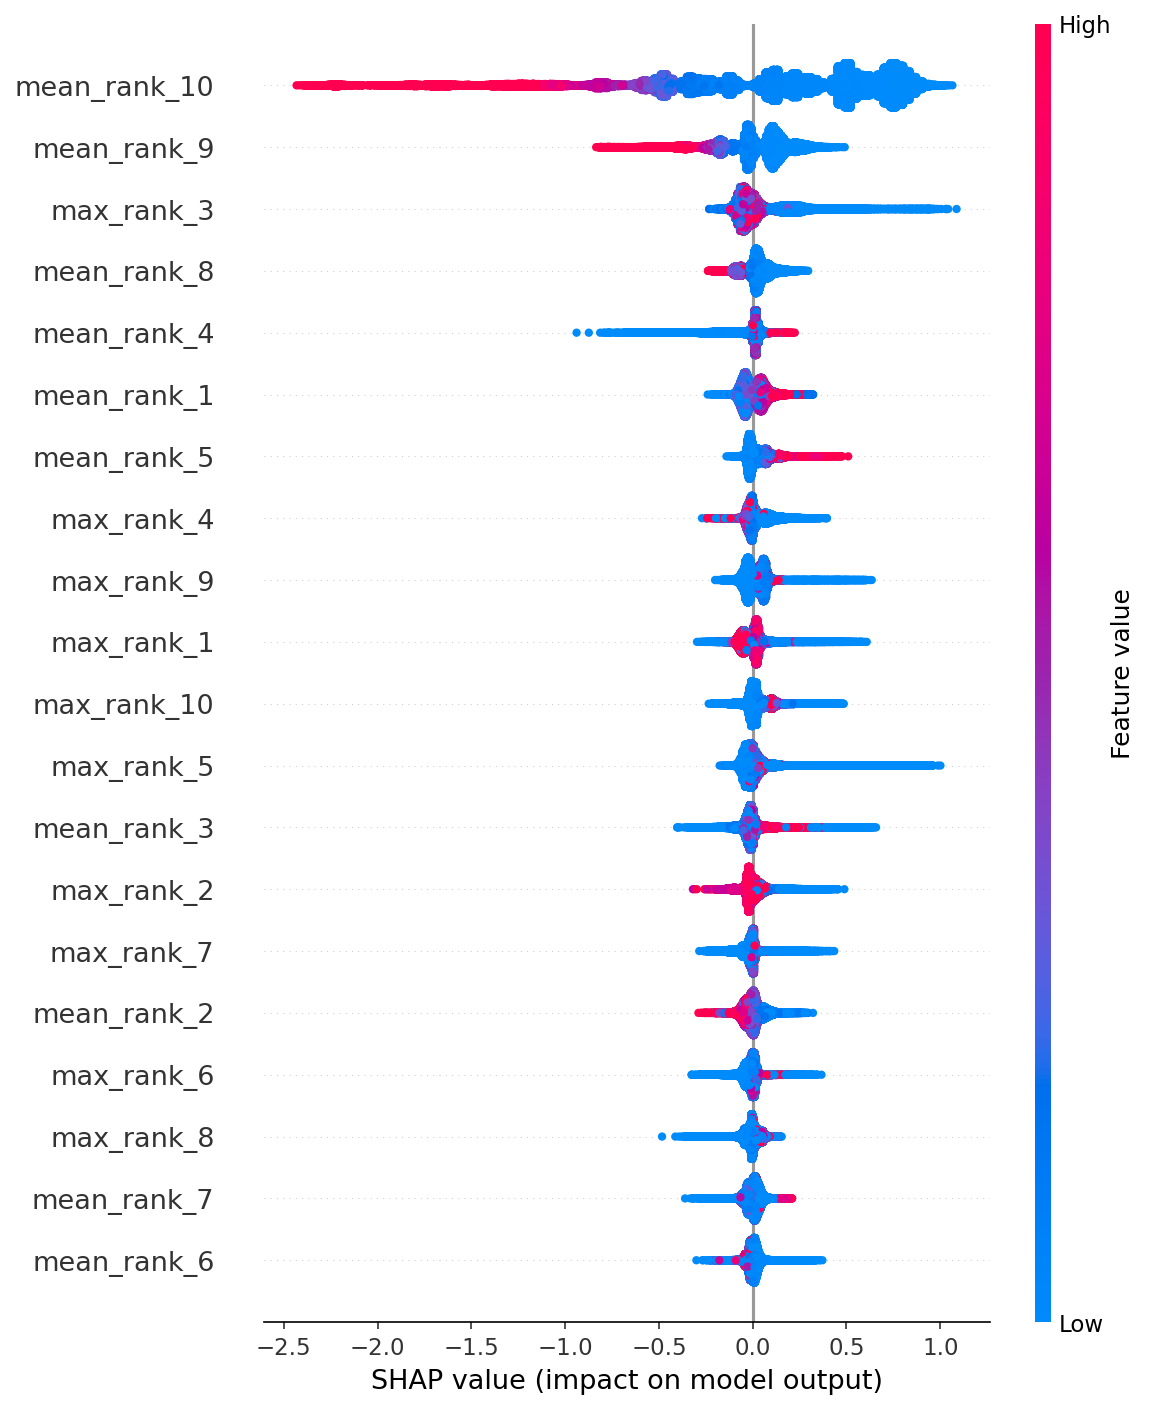
\includegraphics[width=0.7\textwidth]{xgb_shap_beeswarm.png}
\caption{\textit{Beeswarm plot} SHAP des features WEPR pour le modèle XGBoost. Chaque point est une observation~; la couleur représente la valeur de la feature (rouge $=$ élevée, bleu $=$ faible). Les valeurs SHAP négatives poussent la prédiction vers \emph{halluciné}.}
\label{fig:shap_beeswarm}
\end{figure}

Cette importance numérique de \texttt{mean\_rank\_10} ne signifie pas pour autant que ce rang soit en lui-même le meilleur signal~: toutes les features \texttt{mean\_rank\_k} sont fortement corrélées entre elles ($\rho > 0{,}97$ entre rangs adjacents), et c'est en réalité \texttt{mean\_rank\_7} qui a la plus forte corrélation univariée avec $y$ ($-0{,}26$). XGBoost choisit \texttt{mean\_rank\_10} pour résumer l'information de la queue de distribution, mais une régression logistique sur \texttt{mean\_rank\_7} seule produirait probablement une AUC comparable. Les détails complets (gain, SHAP par feature, mises en garde sur la multicolinéarité) figurent en annexe~\ref{ann:xgb}.

\subsection{Synthèse}

WEPR améliore la détection d'erreurs par rapport aux approches non supervisées, et son extension non linéaire par XGBoost en tire encore $+2{,}5$ points d'AUC. Cependant, les performances restent modérées (AUC $\simeq 0{,}68$--$0{,}71$). Cette borne reflète la difficulté intrinsèque du problème : les distributions top-$K$ contiennent un signal réel mais limité, dont l'exploitation maximale nécessiterait des sources d'information complémentaires.

% =============================================================================
% Section 5 — Comparaison transverse
% =============================================================================

\section{Comparaison transverse et transfert des méthodes}
\label{sec:transverse}

\subsection{Motivation et trois ponts}

Chaque section précédente a étudié un couple particulier (méthode, dataset). Pour évaluer la robustesse des méthodes, nous établissons trois ponts~: (i)~appliquer WEPR aux générations CoT de GSM8K~; (ii)~appliquer l'\emph{entropie sémantique} (Kuhn et al., 2023) à TriviaQA-numérique~; (iii)~construire une table croisée scores~$\times$~datasets unifiant les trois sections.

\subsection{Transfert de WEPR à GSM8K}
\label{sec:transfert_wepr}

Réentraîné sur GSM8K (avec $K=10$, exactitude $96{,}1\%$, $n=1\,319$), WEPR atteint AUC $= 0{,}726$ sur la génération complète, soit le même niveau que la régression à 64 variables manuelles de la section~\ref{sec:generations_longues} ($0{,}729$)~: la représentation top-$K$ encode déjà l'essentiel du signal capté manuellement. Sur le sous-ensemble aligné de 300 questions (utilisé dans la table croisée), WEPR atteint AUC $= 0{,}922$, contre $0{,}804$ pour la perplexité~: l'écart de $+12$ points est nettement plus marqué que sur TriviaQA-WEPR ($+5$ points). \emph{Le bénéfice marginal de WEPR croît avec la longueur des séquences générées.}

Le tableau~\ref{tab:transfer_wepr} évalue la transférabilité du modèle. L'asymétrie est complète~: WEPR-TriviaQA appliqué à GSM8K atteint $0{,}79$, soit une performance \emph{supérieure} à son in-domain ($0{,}68$, effet de prévalence). À l'inverse, WEPR-GSM8K appliqué à TriviaQA s'effondre à $0{,}48$, en-dessous du hasard~: les coefficients sont d'amplitude beaucoup plus grande ($|6{,}77|$ contre $|0{,}56|$), symptôme d'un sur-ajustement aux 51 erreurs disponibles. \emph{Un détecteur WEPR appris sur un grand corpus diversifié est transférable~; appris sur un petit corpus déséquilibré, il ne l'est pas.}

\begin{table}[H]
\centering
\caption{Transfert de WEPR — AUC selon le couple (modèle, dataset d'évaluation).}
\label{tab:transfer_wepr}
\small
\begin{tabular}{lcc}
\toprule
                              & Éval.\ TriviaQA & Éval.\ GSM8K \\
\midrule
Modèle TriviaQA               & $\mathbf{0{,}681}$ (in-dom.) & $0{,}793$ \\
Modèle GSM8K                  & $0{,}477$ & $\mathbf{0{,}829}$ (in-dom.) \\
\bottomrule
\end{tabular}
\end{table}

\subsection{Entropie sémantique appliquée à TriviaQA-numérique}

Pour chaque question, nous générons $K=5$ réponses à $T=1{,}0$, regroupées par identité numérique au seuil près. L'entropie sémantique est $\mathrm{SE} = -\sum_c P(c)\log P(c)$, où $P(c)$ est pondéré par la log-probabilité moyenne des réponses du cluster $c$.

Sur 2\,574 questions, $94{,}8\%$ ont $\mathrm{SE} = 0$ (les 5 réponses coïncident). La SE moyenne diffère d'un facteur 17 entre correctes ($0{,}013$) et incorrectes ($0{,}224$), avec une corrélation de Spearman de $+0{,}43$ avec l'erreur absolue. Mais l'AUC de SE n'est que de $0{,}65$, contre $\sim 0{,}86$ pour les meilleures log-probabilités~: les ex-aequo massifs à $\mathrm{SE}=0$ pénalisent l'AUC tout en étant absorbés correctement par Spearman. \textbf{SE et log-probabilités mesurent des aspects différents}~: la première capture l'\emph{instabilité externe} entre échantillons indépendants, les secondes la \emph{concentration locale} sur la propre génération du modèle. Nous identifions des questions où la probabilité jointe est proche de $1$ et où le modèle produit pourtant 5 réponses différentes à $T=1$~: les deux signaux sont \emph{complémentaires}.

\subsection{Table croisée et lectures transverses}
\label{sec:cross_table}

La figure~\ref{fig:cross_heatmap} présente l'AUC de discrimination correct/incorrect pour chaque couple score~$\times$~dataset.

\begin{figure}[H]
\centering

\includegraphics[width=0.78\textwidth]{figures/cross_auc_heatmap.pdf}
\caption{AUC de discrimination correct/incorrect, scores~$\times$~datasets. Les cellules grises indiquent un score non applicable au dataset.}
\label{fig:cross_heatmap}
\end{figure}

Trois observations émergent. Premièrement, \emph{aucune hiérarchie n'est universelle}~: la perplexité domine sur TriviaQA-num ($\sim 4$ tokens, AUC $> 0{,}85$) tandis que WEPR domine sur GSM8K ($\sim 188$ tokens, AUC $0{,}92$). Deuxièmement, $P_{\mathrm{joint}}$ chute de $0{,}86$ à $0{,}64$ entre TriviaQA-num et TriviaQA-WEPR (mêmes données, filtre numérique vs textuel)~: le produit $\prod_t p_t$ s'écrase mécaniquement vers zéro dès quelques tokens, phénomène invisible section par section. Troisièmement, ELI5 ressort comme le régime le plus difficile~: aucun score ne dépasse $0{,}66$ d'AUC, ce qui définit une borne empirique de difficulté liée au caractère subjectif de la vérité dans ce dataset.

\paragraph{Calibration.}
Le tableau~\ref{tab:cross_ece} reporte l'\emph{Expected Calibration Error}. WEPR atteint sur TriviaQA-WEPR une ECE de $0{,}009$ — quasi parfaite — car il sort directement la probabilité d'une régression logistique optimisée par log-loss. À l'inverse, $P_{\mathrm{joint}}$ atteint une ECE de $0{,}97$ sur GSM8K~: \emph{$P_{\mathrm{joint}}$ ne doit pas être interprétée comme une probabilité au-delà de quelques tokens.}

\begin{table}[H]
\centering
\caption{ECE (10 bins) des scores interprétables comme probabilités.}
\label{tab:cross_ece}
\small
\begin{tabular}{lcccc}
\toprule
Score & TriviaQA-num & TriviaQA-WEPR & GSM8K & ELI5 \\
\midrule
$P_{\mathrm{joint}}$  & $0{,}096$ & $0{,}384$ & $0{,}969$ & $0{,}820$ \\
$P_{\mathrm{geo}}$    & $0{,}103$ & $0{,}074$ & $0{,}082$ & $0{,}063$ \\
$p_{\min}$            & $0{,}097$ & $0{,}297$ & $0{,}862$ & $0{,}524$ \\
WEPR                  & $0{,}030$ & $\mathbf{0{,}009}$ & $0{,}245$ & $0{,}687$ \\
\bottomrule
\end{tabular}
\end{table}

\subsection{Comparaison aux résultats de la littérature}
\label{sec:comp_litterature}

Nos résultats peuvent être confrontés à ceux des papiers de référence. La comparaison reste indicative car les datasets, les modèles et les protocoles d'annotation diffèrent~; nous insistons sur les ordres de grandeur et la cohérence qualitative.

\paragraph{Confiance verbalisée et white-box (Xiong et al.\ 2024).}
\citet{xiong2024} reportent sur leurs huit datasets (GSM8K, SVAMP, DateUnd, etc.\ -- \emph{pas} TriviaQA) une AUROC moyenne de la confiance verbalisée \textit{vanilla} comprise entre $0{,}51$ (GPT-3) et $0{,}63$ (GPT-4), et un gain typique des méthodes white-box plafonnant à $0{,}52$--$0{,}60$. Nous obtenons sur TriviaQA-num une AUROC de $\sim 0{,}68$ pour la confiance verbalisée (Gemini~2.0~Flash) et $\sim 0{,}86$ pour la probabilité géométrique sur les tokens de la réponse, soit nettement au-dessus de leurs valeurs. L'écart s'explique principalement par le dataset~: TriviaQA-numérique conserve des questions factuelles courtes pour lesquelles le signal log-probabiliste est particulièrement concentré, alors que les benchmarks de raisonnement utilisés par Xiong et al.\ sont structurellement plus difficiles à classer. La hiérarchie qualitative est en revanche conforme~: la confiance verbalisée est moins discriminante que les signaux internes, et toutes les méthodes souffrent d'une surconfiance systématique.

\paragraph{Prédiction conforme (Ye et al.\ 2024).}
\citet{ye2024benchmarking} évaluent LAC et APS à $\alpha = 0{,}10$ sur cinq benchmarks (dont MMLU) avec 9 familles de LLMs. Dans leur tableau principal (Section~6.1), les chiffres reportés sont la moyenne LAC$+$APS pour atténuer l'effet du choix du score de non-conformité~; les valeurs séparées figurent dans leur Annexe~C.1. Pour Qwen-14B sur la tâche QA (MMLU), ils rapportent LAC~: $\mathrm{CR} = 90{,}43\%$, $\mathrm{SS} = 2{,}39$~; APS~: $\mathrm{CR} = 94{,}74\%$, $\mathrm{SS} = 3{,}21$. Le papier indique explicitement que LAC \emph{« can undercover hard instances and overcover easy ones »}, qu'APS \emph{« suffers from, on average, larger prediction sets »}, et qu'\emph{« APS tends to achieve higher coverage rates than LAC due to its larger prediction sets in most cases »}~: l'observation qualitative que APS sur-couvre et produit des ensembles plus grands est donc directement reprise du papier. Sur nos 107 questions MMLU avec Gemini, nos chiffres LAC ($\mathrm{CR} \sim 0{,}88$, $\mathrm{SS} \sim 1{,}5$) et la sur-couverture relative d'APS sont cohérents avec ce schéma. Notre légère sous-couverture LAC sous la cible $0{,}90$ s'explique par le faible nombre de calibration ($\sim 50$ obs.), bien en deçà de leurs $10\,000$ instances par tâche.

\paragraph{WEPR (Moslonka et al.\ 2025).}
\citet{moslonka2026} reportent sur TriviaQA des AUC de WEPR comprises entre $0{,}82$ (Mistral-Small-24B) et $0{,}86$ (Phi-4, Ministral-8B), avec un gain WEPR$-$EPR de $+4$ à $+7$ points. Nos chiffres correspondants sont $\mathrm{AUC}_{\text{WEPR}} = 0{,}682$ et $\mathrm{AUC}_{\text{EPR}} = 0{,}656$, avec un gain de $+2{,}6$ points~: les AUC absolues sont sensiblement plus basses, et le gain marginal plus modeste. Deux raisons probables. D'une part, le modèle utilisé diffère (Gemini~2.0~Flash chez nous, Mistral / Phi / Ministral chez eux)~: notre LLM est plus petit, ce qui peut affecter à la fois la qualité brute des réponses et la structure des distributions top-$K$. D'autre part, le protocole d'annotation diffère~: \citet{moslonka2026} utilisent un appariement à des réponses de référence multiples, alors que nous utilisons un juge LLM unique, ce qui produit un déséquilibre de classes ($84{,}7\%$ de correctes) plus marqué que dans leur protocole et peut limiter la marge d'amélioration apportée par l'apprentissage supervisé. Nous avons par ailleurs repris la valeur $K=10$ utilisée par \citet{moslonka2026}, qui rapportent un plateau de performance autour de $K \approx 8$--$10$ rangs accessibles. Nous n'avons pas conduit d'analyse de sensibilité propre sur cet hyperparamètre~: tester $K \in \{5, 8, 10, 15\}$ pour vérifier indépendamment l'existence et la position du plateau sur notre cadre constitue un prolongement naturel.

\paragraph{SelfCheckGPT (Manakul et al.\ 2023).}
\citet{manakul2023selfcheckgpt} évaluent leurs cinq variantes sur WikiBio (passages biographiques GPT-3 annotés au niveau phrase). Les meilleures variantes atteignent une AUC-PR (NonFact) de $93{,}4\%$ pour SelfCheck-Prompt et $92{,}5\%$ pour SelfCheck-NLI, contre $87{,}5\%$ pour la baseline grey-box Max($-\log p$). La tâche n'est pas directement comparable à nos expériences (factualité phrase-par-phrase sur des biographies, vs détection d'erreur sur réponse courte). Nous nous limitons à reprendre l'\emph{intuition centrale} -- l'instabilité entre échantillons indépendants comme signal d'incertitude -- via l'entropie sémantique de \citet{kuhn2023semantic} appliquée à TriviaQA-num. Sur ce cadre, notre AUC SE de $0{,}65$ et la corrélation Spearman de $+0{,}43$ avec l'erreur absolue confirment qualitativement leur résultat~: la cohérence entre générations capture une dimension d'incertitude que les log-probabilités locales manquent.

\paragraph{Synthèse de la comparaison.}
Trois constats émergent. Premièrement, les hiérarchies qualitatives observées dans la littérature se retrouvent dans notre travail (verbalisée $<$ white-box $<$ supervisée multi-features pour la détection~; APS plus conservateur que LAC). Deuxièmement, les AUC absolues dépendent fortement du couple (modèle, dataset)~: nos chiffres sur TriviaQA-num sont \emph{plus élevés} que ceux de Xiong et al., et nos chiffres WEPR sur TriviaQA-WEPR sont \emph{plus bas} que ceux de Moslonka et al. Cette double divergence interdit toute conclusion absolue mais souligne que la quantification d'incertitude est sensible au régime de génération. Troisièmement, les phénomènes que nous mettons au jour -- l'effondrement de $P_{\mathrm{joint}}$ avec la longueur, l'asymétrie du transfert WEPR entre datasets, la complémentarité log-probabilités / entropie sémantique -- ne sont pas explicitement traités dans les papiers cités, et constituent les apports propres de notre dispositif transverse.

% ========================================
% CONCLUSION
% ========================================

\section{Conclusion}

Au-delà de la juxtaposition des sections, ce travail dégage un cadre articulé autour de \emph{trois échelles d'incertitude}. À l'\textbf{échelle locale du token}, la distribution sur le prochain token discrimine très bien sur des sorties courtes (AUC $> 0{,}85$ sur TriviaQA-num) mais sature sur les générations longues (probabilité jointe écrasée vers zéro) et n'est jamais directement calibrée. À l'\textbf{échelle structurelle de la séquence}, la dynamique de l'incertitude (entropie en fin de génération, distributions top-$K$) est exploitée par WEPR qui atteint AUC $= 0{,}92$ sur GSM8K. À l'\textbf{échelle externe de l'instabilité entre échantillons}, l'entropie sémantique distingue fortement les réponses incorrectes (SE moyenne $\times 17$) et capture une dimension complémentaire des log-probabilités internes.

\paragraph{Ce qui fonctionne.} Les log-probabilités internes contiennent un signal réel sur la fiabilité, plus fort que les scores verbalisés. Les réponses incorrectes sont associées à une incertitude plus instable, en particulier dans les dernières étapes de la génération. Une combinaison supervisée (WEPR) dépasse systématiquement les approches univariées sur les générations longues, et son entraînement sur un grand corpus diversifié produit un détecteur transférable. La prédiction conforme fournit des garanties rigoureuses pour les QCM.

\paragraph{Limitations.} Les performances restent modérées (AUC $0{,}68$--$0{,}73$ sur la détection d'erreurs dans TriviaQA), loin de la perfection nécessaire pour un déploiement non supervisé. Les scores verbalisés sont structurellement mal calibrés (moyenne $0{,}96$ vs exactitude $0{,}86$). Les performances chutent fortement sur les tâches à vérité subjective (ELI5).

\paragraph{Perspectives.} Quatre pistes naturelles se dégagent~: (i)~combiner les features WEPR et l'entropie sémantique, qui mesurent des dimensions complémentaires~; (ii)~explorer des modèles non linéaires plus expressifs sur les distributions top-$K$~; (iii)~tester la transférabilité inter-modèles (un détecteur entraîné sur Gemini fonctionne-t-il sur GPT-4 ou Claude ?)~; (iv)~passer d'une détection passive à des approches interventionnelles (décodage contraint, sampling guidé par un détecteur, rejet conditionnel à la prédiction conforme). Le chemin vers des LLMs vraiment dignes de confiance passe par une meilleure articulation de ces différentes échelles d'incertitude avec des sources d'information complémentaires (vérification factuelle, contraintes de décodage, feedback humain).

\newpage

% ========================================
% ANNEXES
% ========================================

\appendix

\section{Statistiques descriptives détaillées des datasets}
\label{ann:datasets}

\subsection{GSM8K}

\begin{figure}[H]
    \centering
    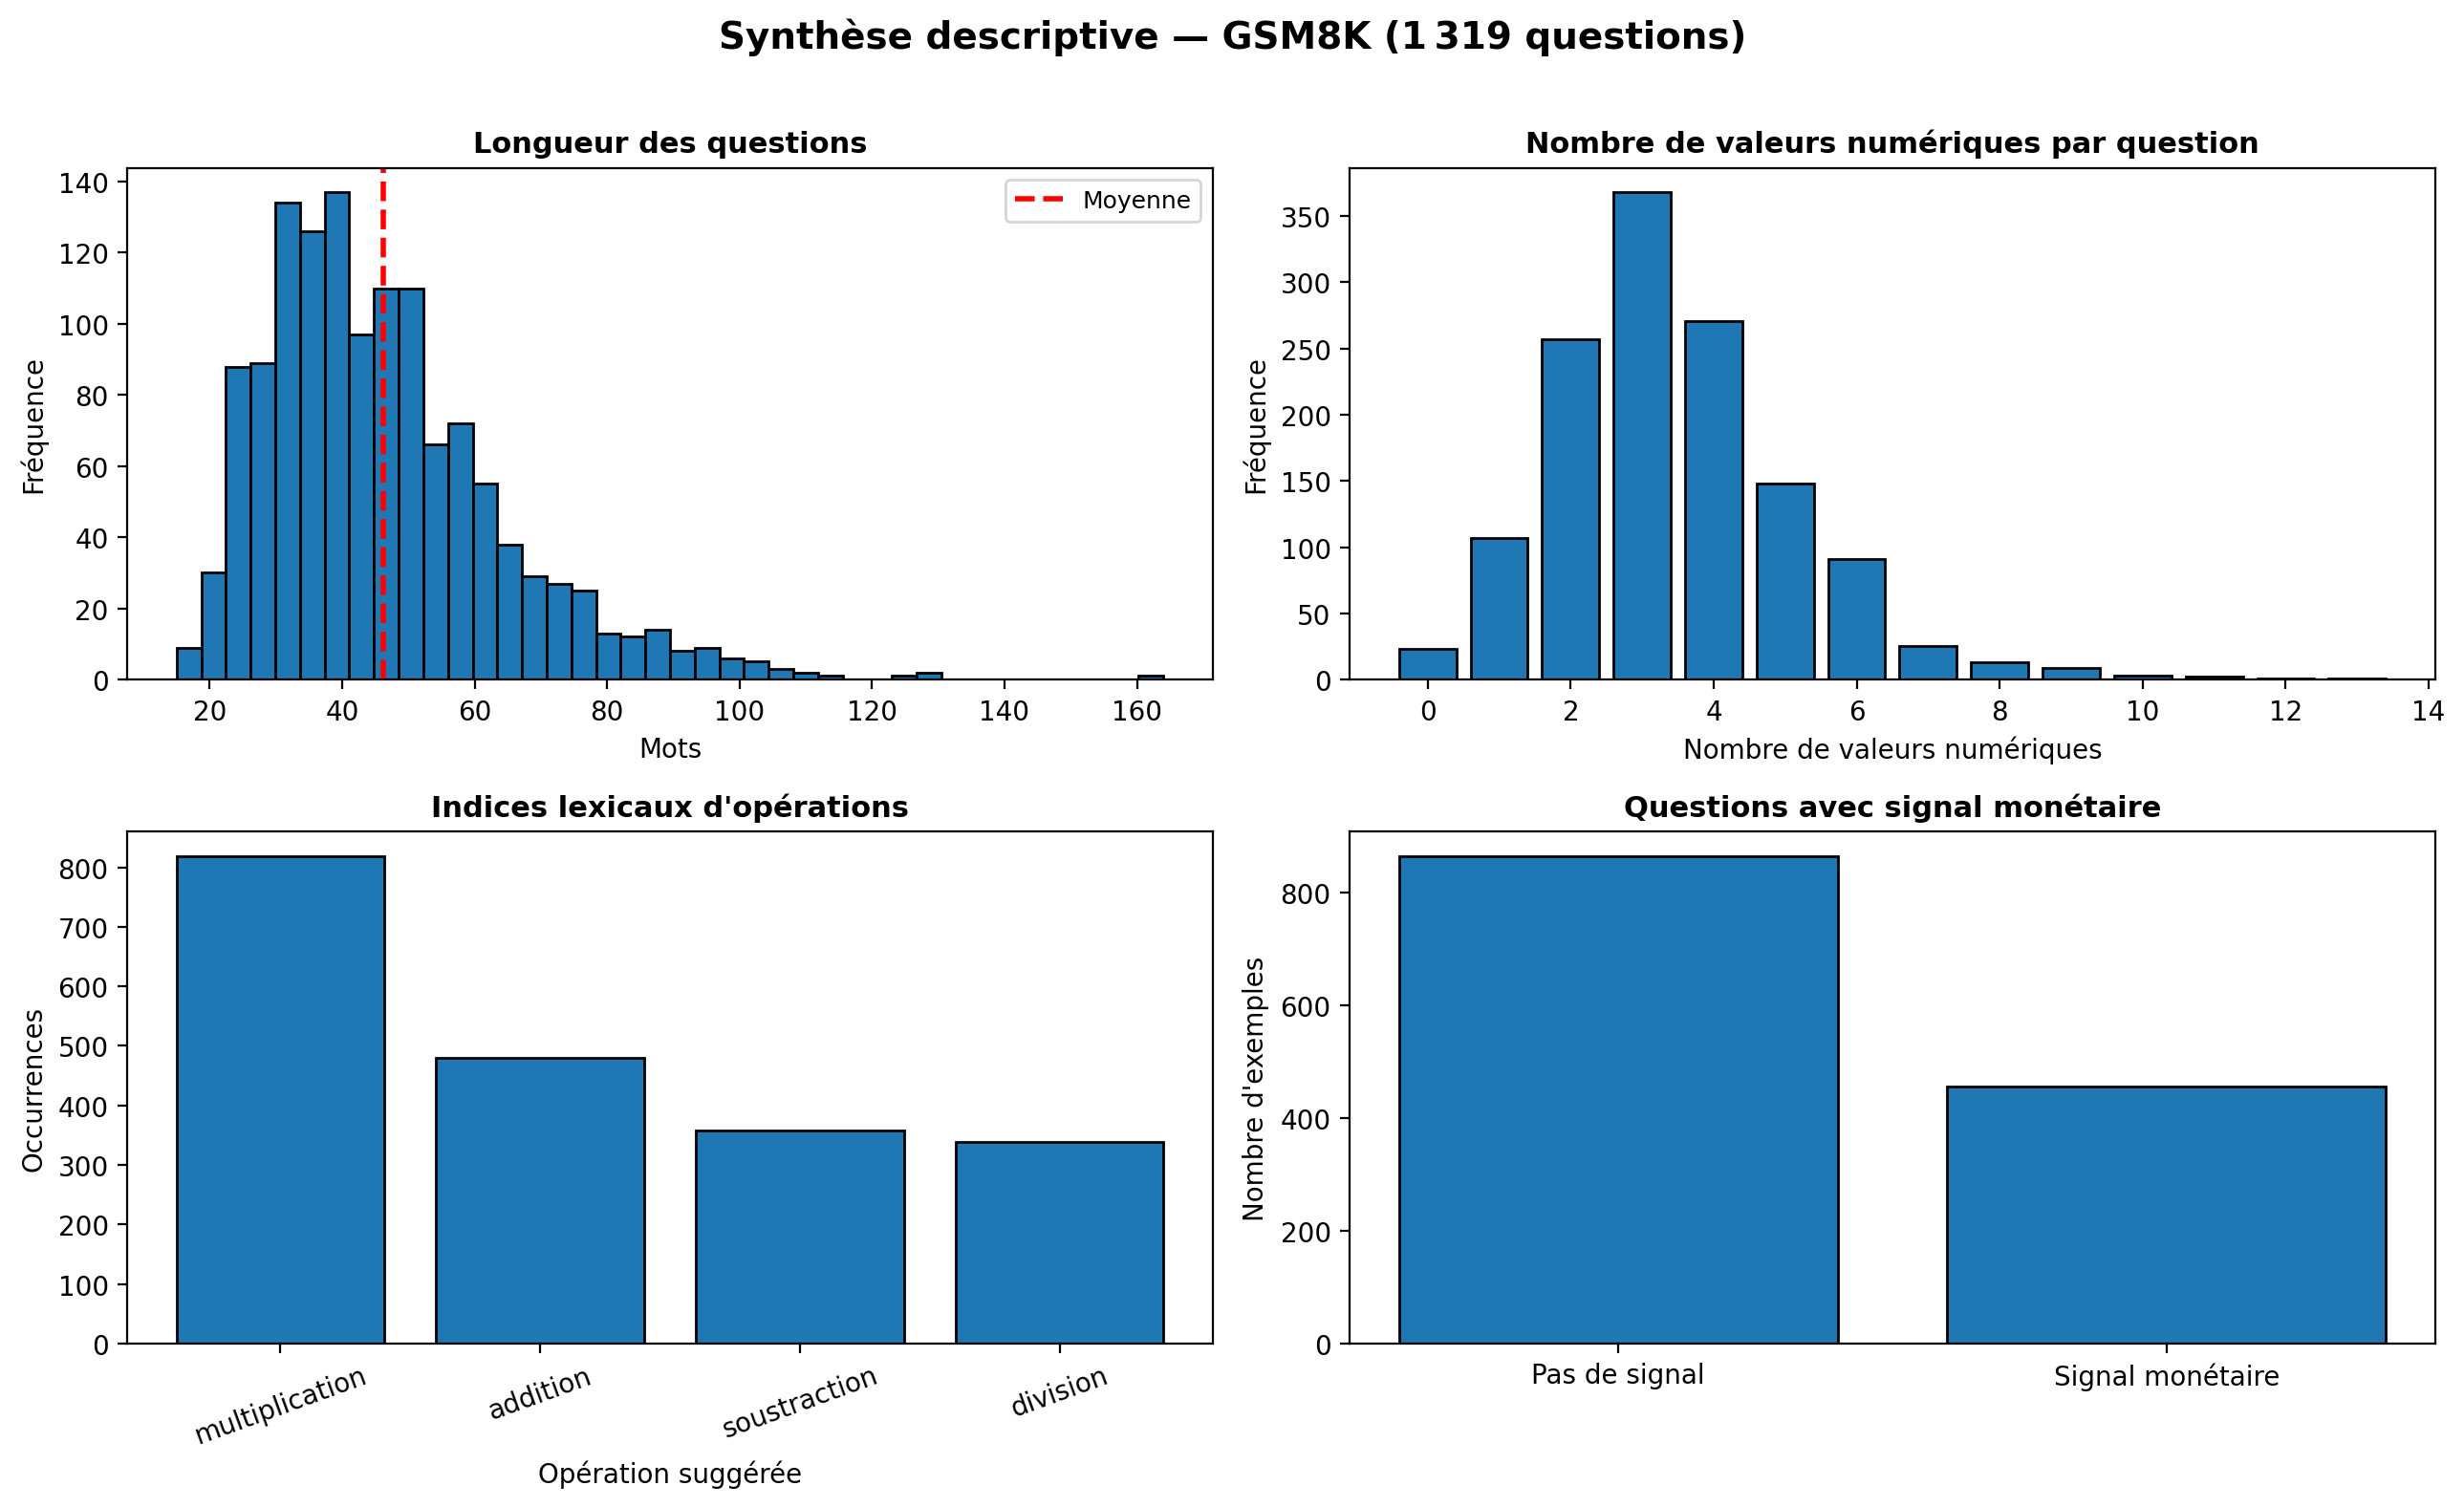
\includegraphics[width=0.95\textwidth]{06_synthese_gsm8k_locale.png}
    \caption{Synthèse descriptive du dataset GSM8K (1\,319 questions).}
    \label{fig:gsm8k_stats}
\end{figure}

\noindent\textbf{Synthèse — GSM8K.} Le split de test contient 1\,319 questions ($\approx 46$ mots en moyenne), avec en moyenne 3{,}5 valeurs numériques par énoncé et un signal monétaire (présence de \texttt{\$}, \emph{dollar}, \emph{cost}, \emph{price}, \emph{pay}\dots) dans 34{,}7\,\% des cas. Les indices d'opérations attendues (additions, soustractions, multiplications, divisions, pourcentages) couvrent l'essentiel des questions, ce qui justifie l'usage de GSM8K comme banc de test d'arithmétique en chaîne. La précision globale du modèle générateur est de 95{,}6\,\% (1\,261/1\,319), laissant 58 erreurs exploitables pour l'analyse de confiance.

\subsection{MMLU}

\begin{figure}[H]
    \centering
    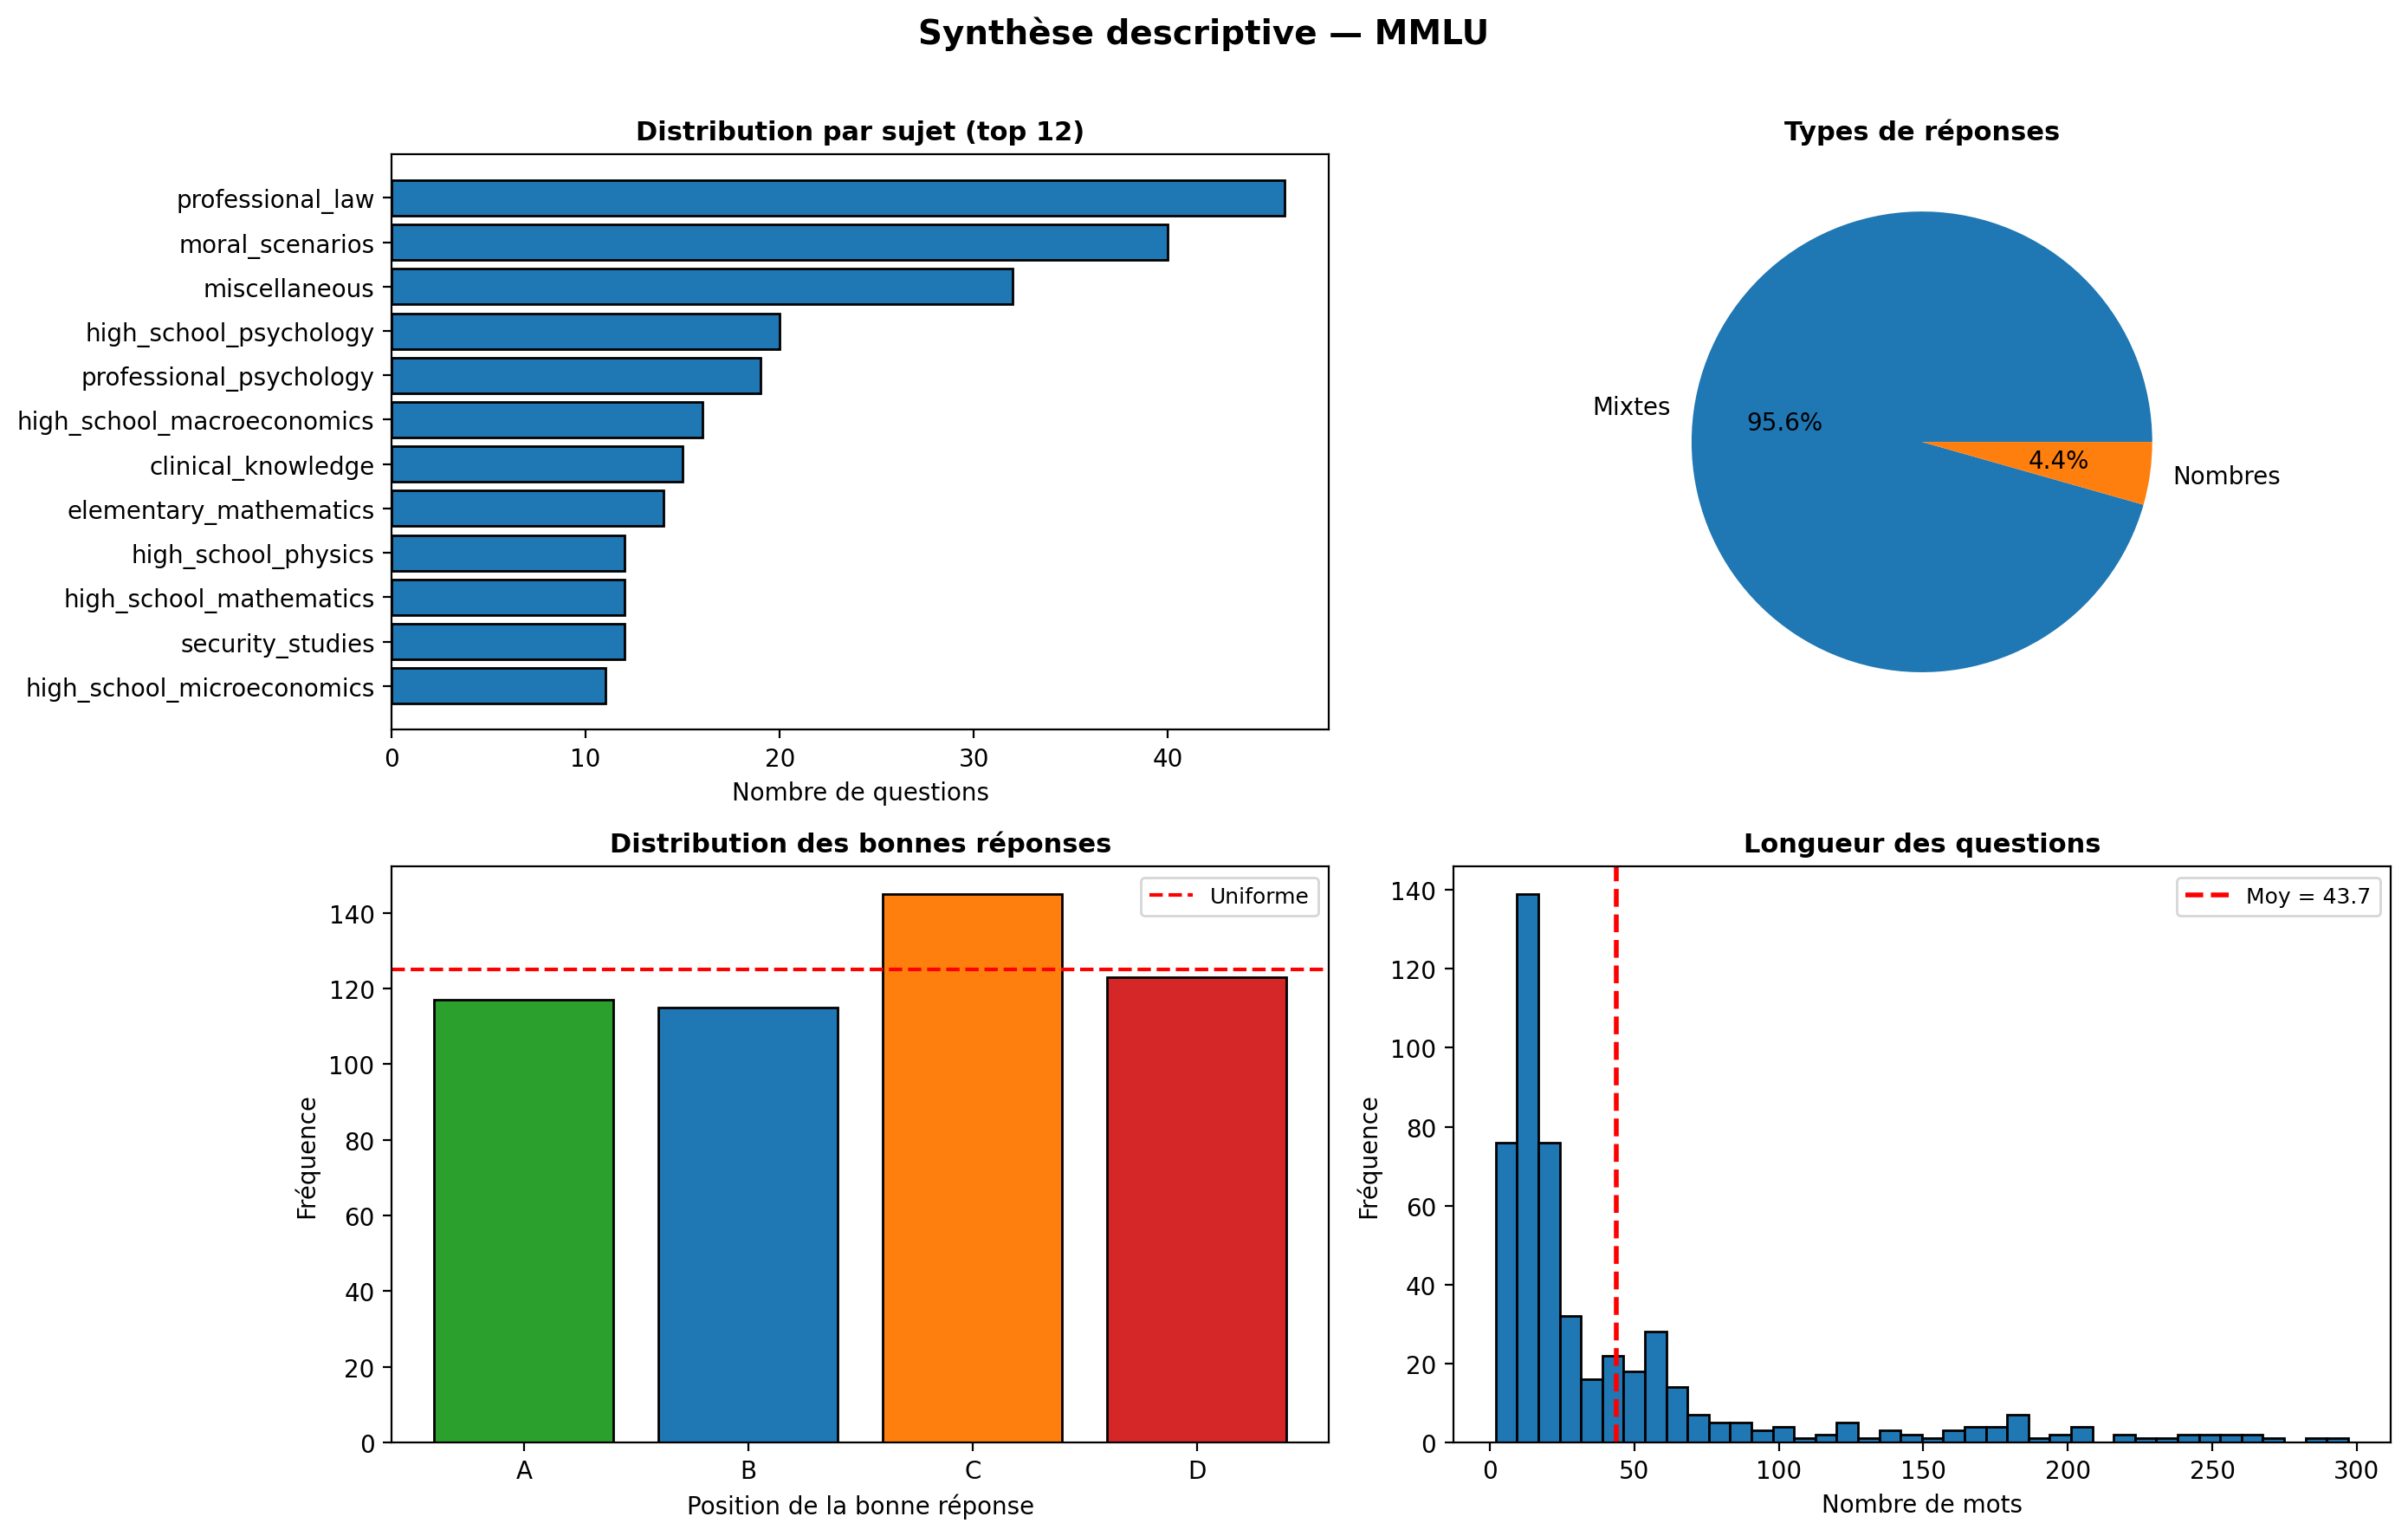
\includegraphics[width=0.95\textwidth]{09_synthese_complete.png}
    \caption{Synthèse descriptive du dataset MMLU.}
    \label{fig:mmlu_stats}
\end{figure}

\noindent\textbf{Synthèse — MMLU.} L'échantillon de référence couvre 57 sujets et 500 questions (longueur moyenne $\approx 44$ mots). La distribution initiale des bonnes réponses parmi $\{A,B,C,D\}$ est légèrement biaisée (sur-représentation de la position D)~; nous appliquons donc une \textbf{permutation aléatoire des choix} avant chaque génération, ce qui ré-uniformise la distribution et garantit que la position de la bonne réponse ne constitue pas un signal exploitable par le modèle (figure~\ref{fig:mmlu_shuffle}). Les sujets les plus représentés sont \emph{professional\_law}, \emph{moral\_scenarios} et \emph{miscellaneous}, ce qui couvre des compétences hétérogènes (raisonnement juridique, dilemmes éthiques, culture générale). Pour la prédiction conforme évaluée en section~\ref{sec:qcm} et l'annexe~\ref{ann:conformal}, on travaille sur un sous-ensemble de 107 questions pour lesquelles les top-$K$ log-probabilités sont disponibles.

\begin{figure}[H]
    \centering
    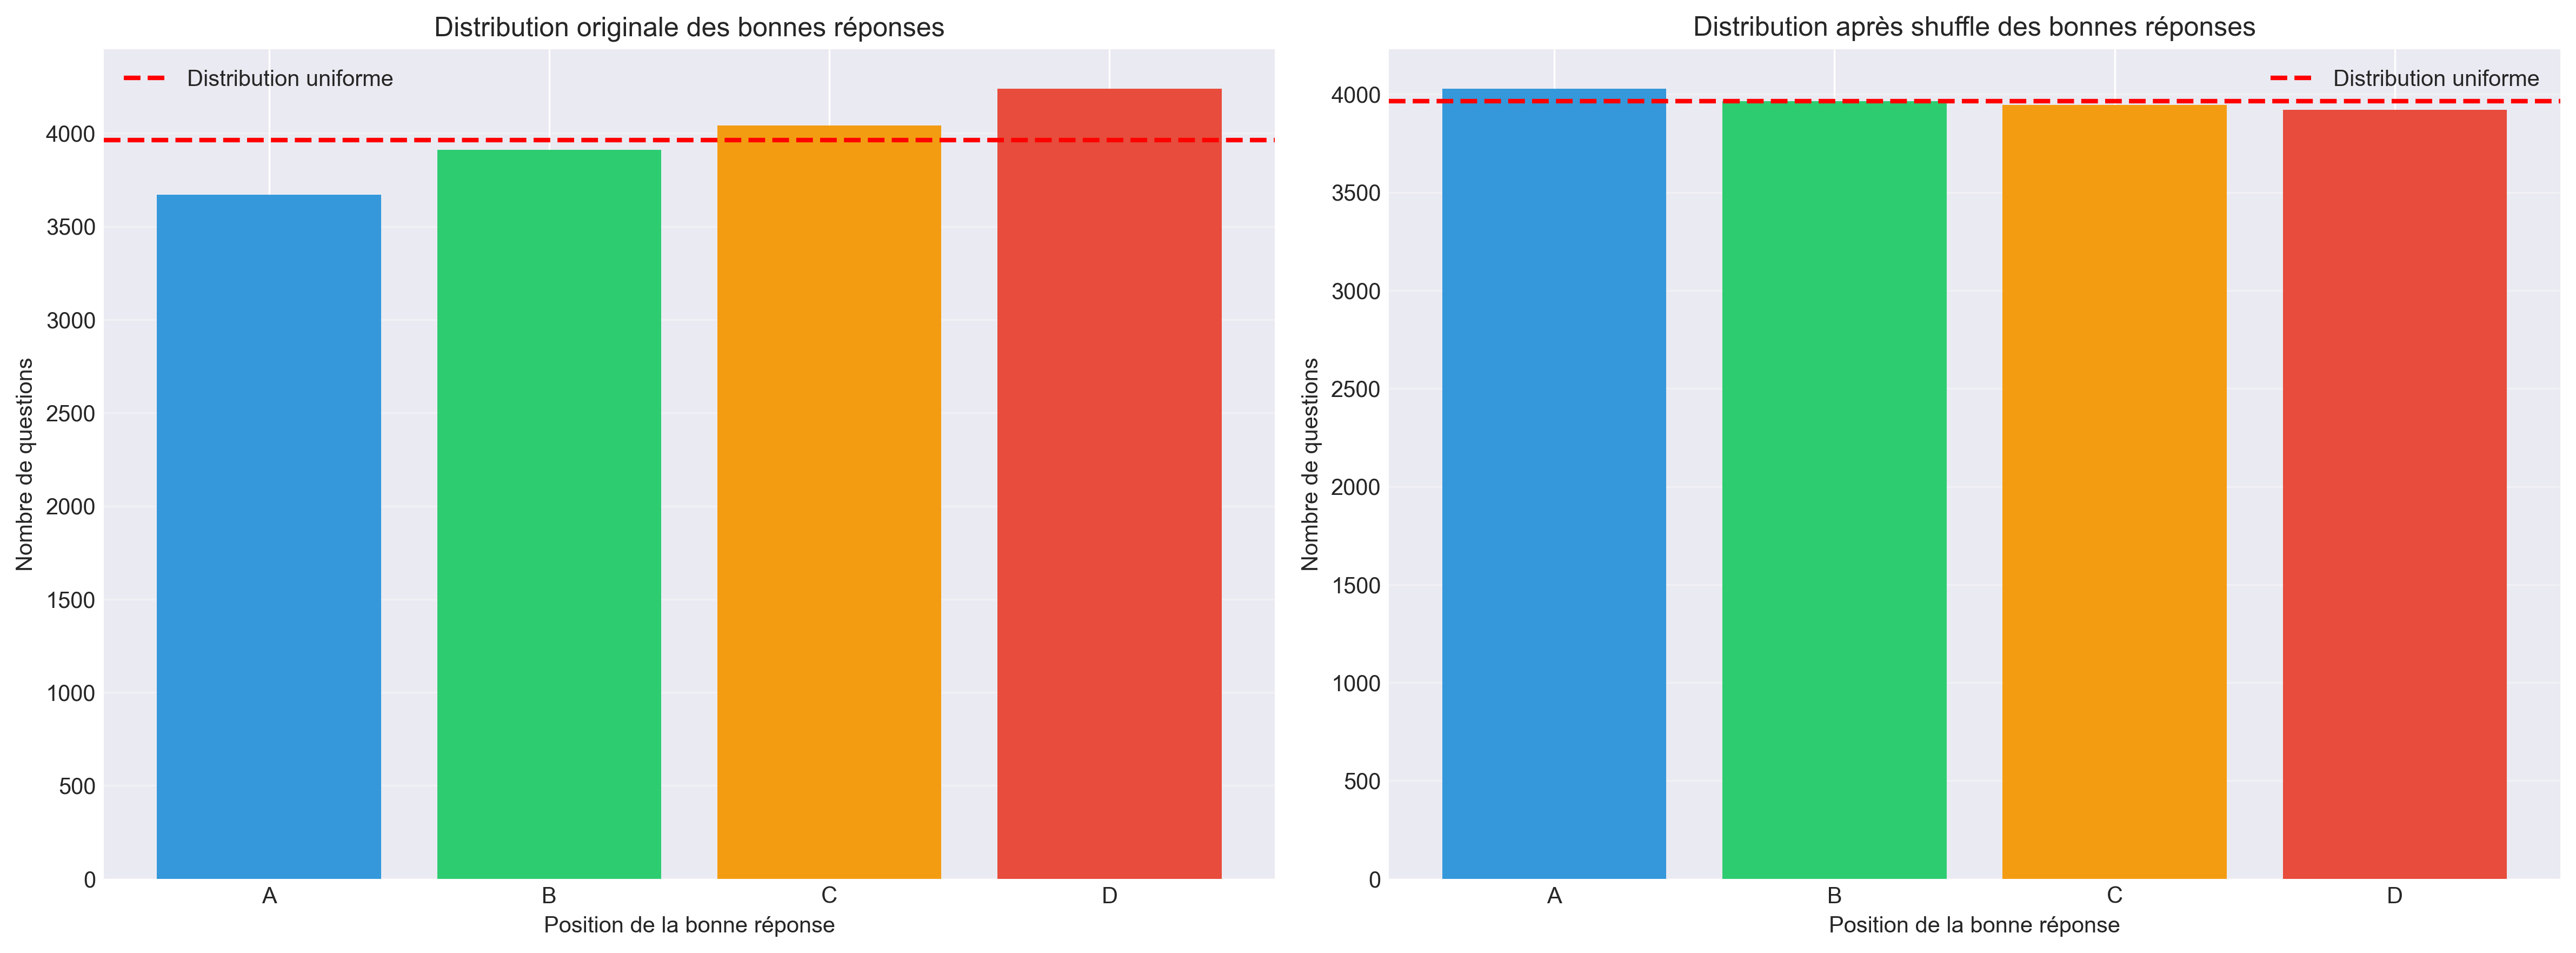
\includegraphics[width=0.95\textwidth]{06_comparaison_shuffle_mmlu.png}
    \caption{Distribution des bonnes réponses sur MMLU avant (gauche) et après (droite) permutation aléatoire des choix. La permutation rétablit une distribution proche de l'uniforme attendue (ligne pointillée).}
    \label{fig:mmlu_shuffle}
\end{figure}

\subsection{TriviaQA}

\begin{figure}[H]
    \centering
    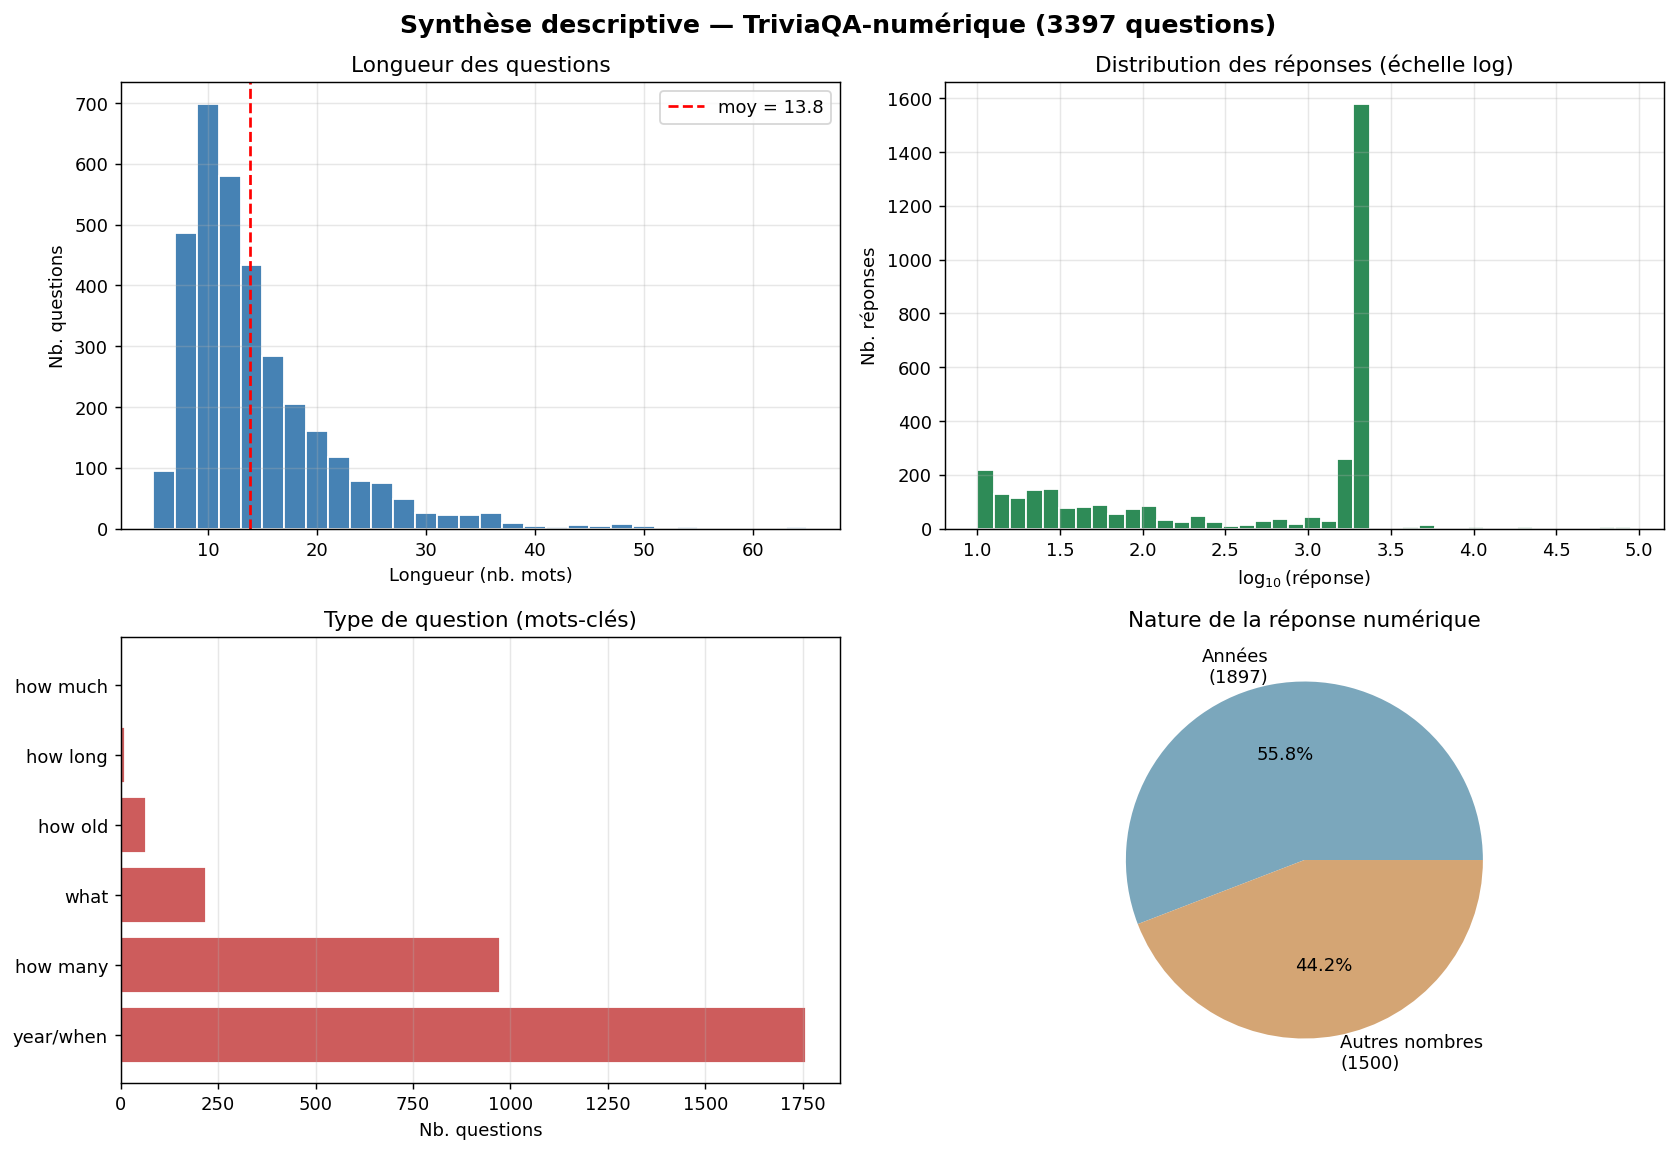
\includegraphics[width=0.95\textwidth]{stats_triviaqa_num.png}
    \caption{Synthèse descriptive de TriviaQA-numérique (3\,397 questions).}
    \label{fig:triviaqa_num_stats}
\end{figure}

\begin{figure}[H]
    \centering
    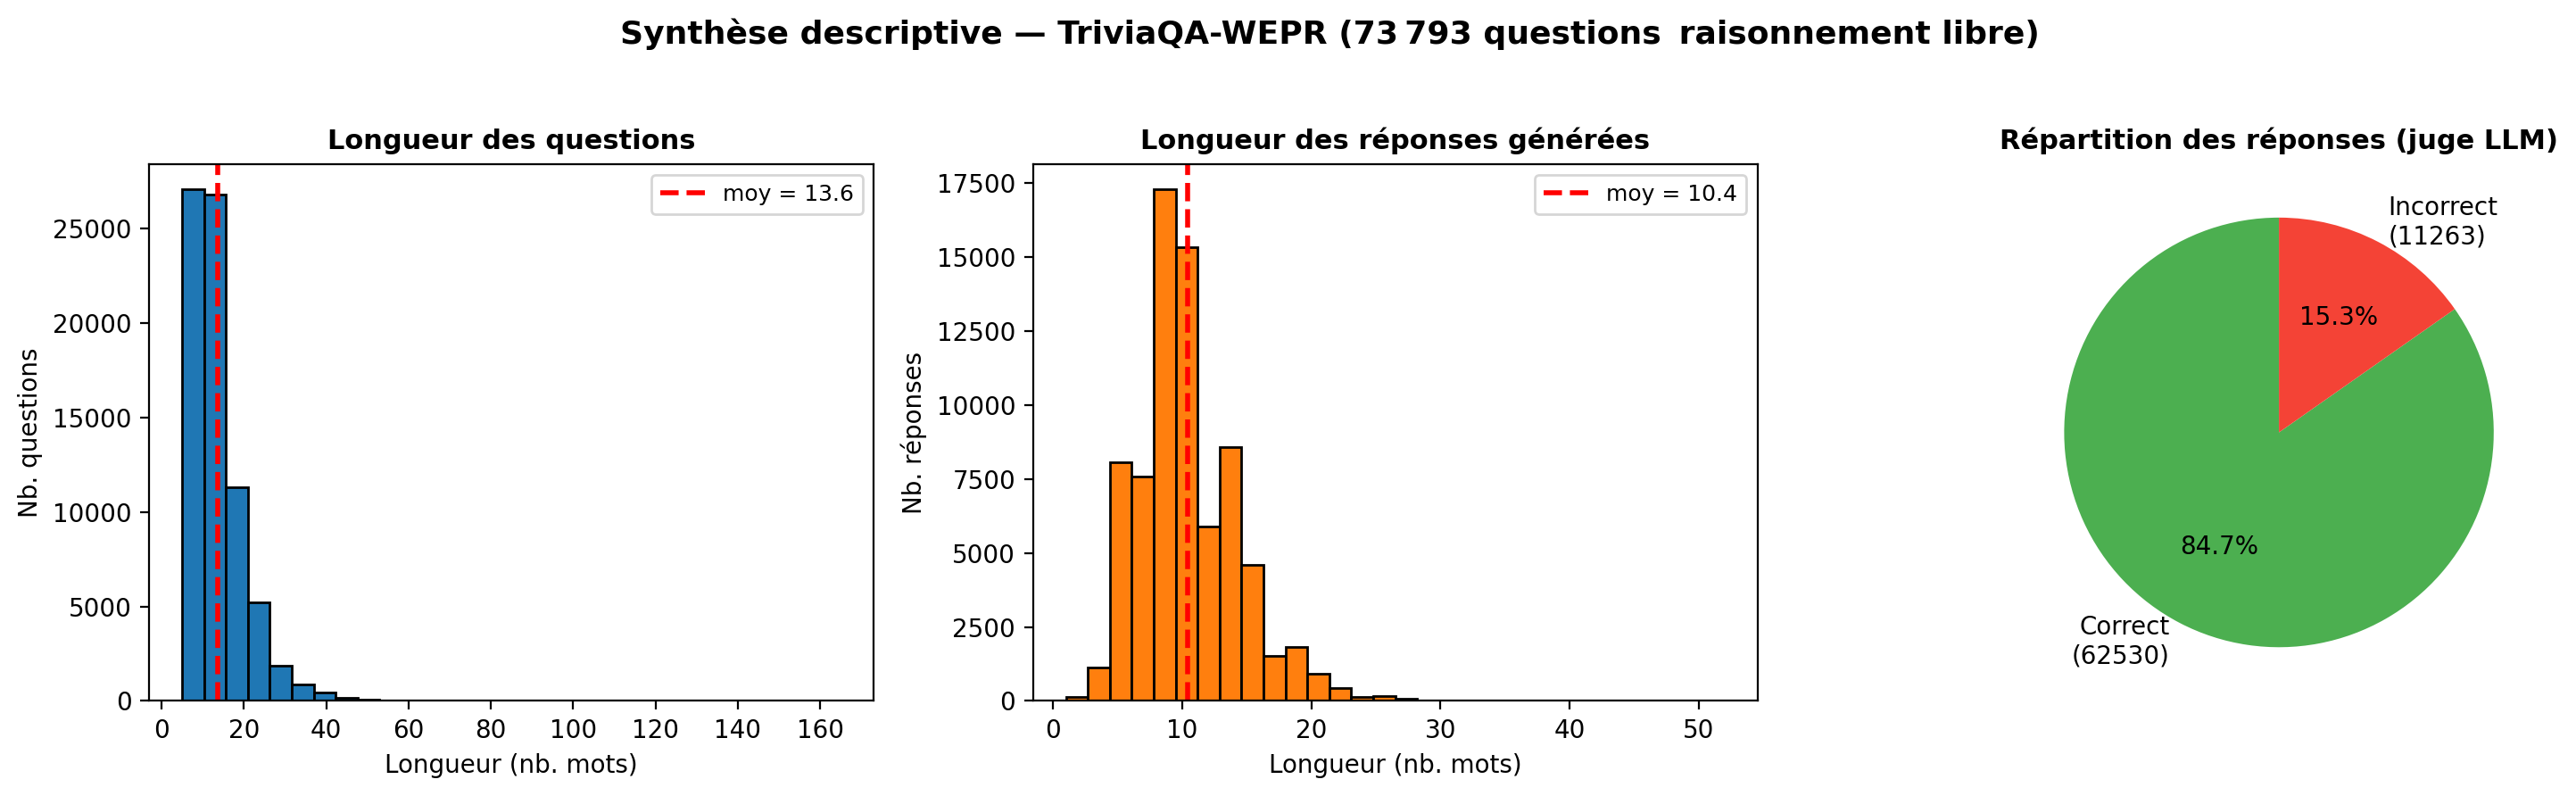
\includegraphics[width=0.95\textwidth]{stats_triviaqa_wepr.png}
    \caption{Synthèse descriptive de TriviaQA-WEPR (73\,793 questions).}
    \label{fig:triviaqa_wepr_stats}
\end{figure}

\subsection{ELI5}

\begin{figure}[H]
    \centering
    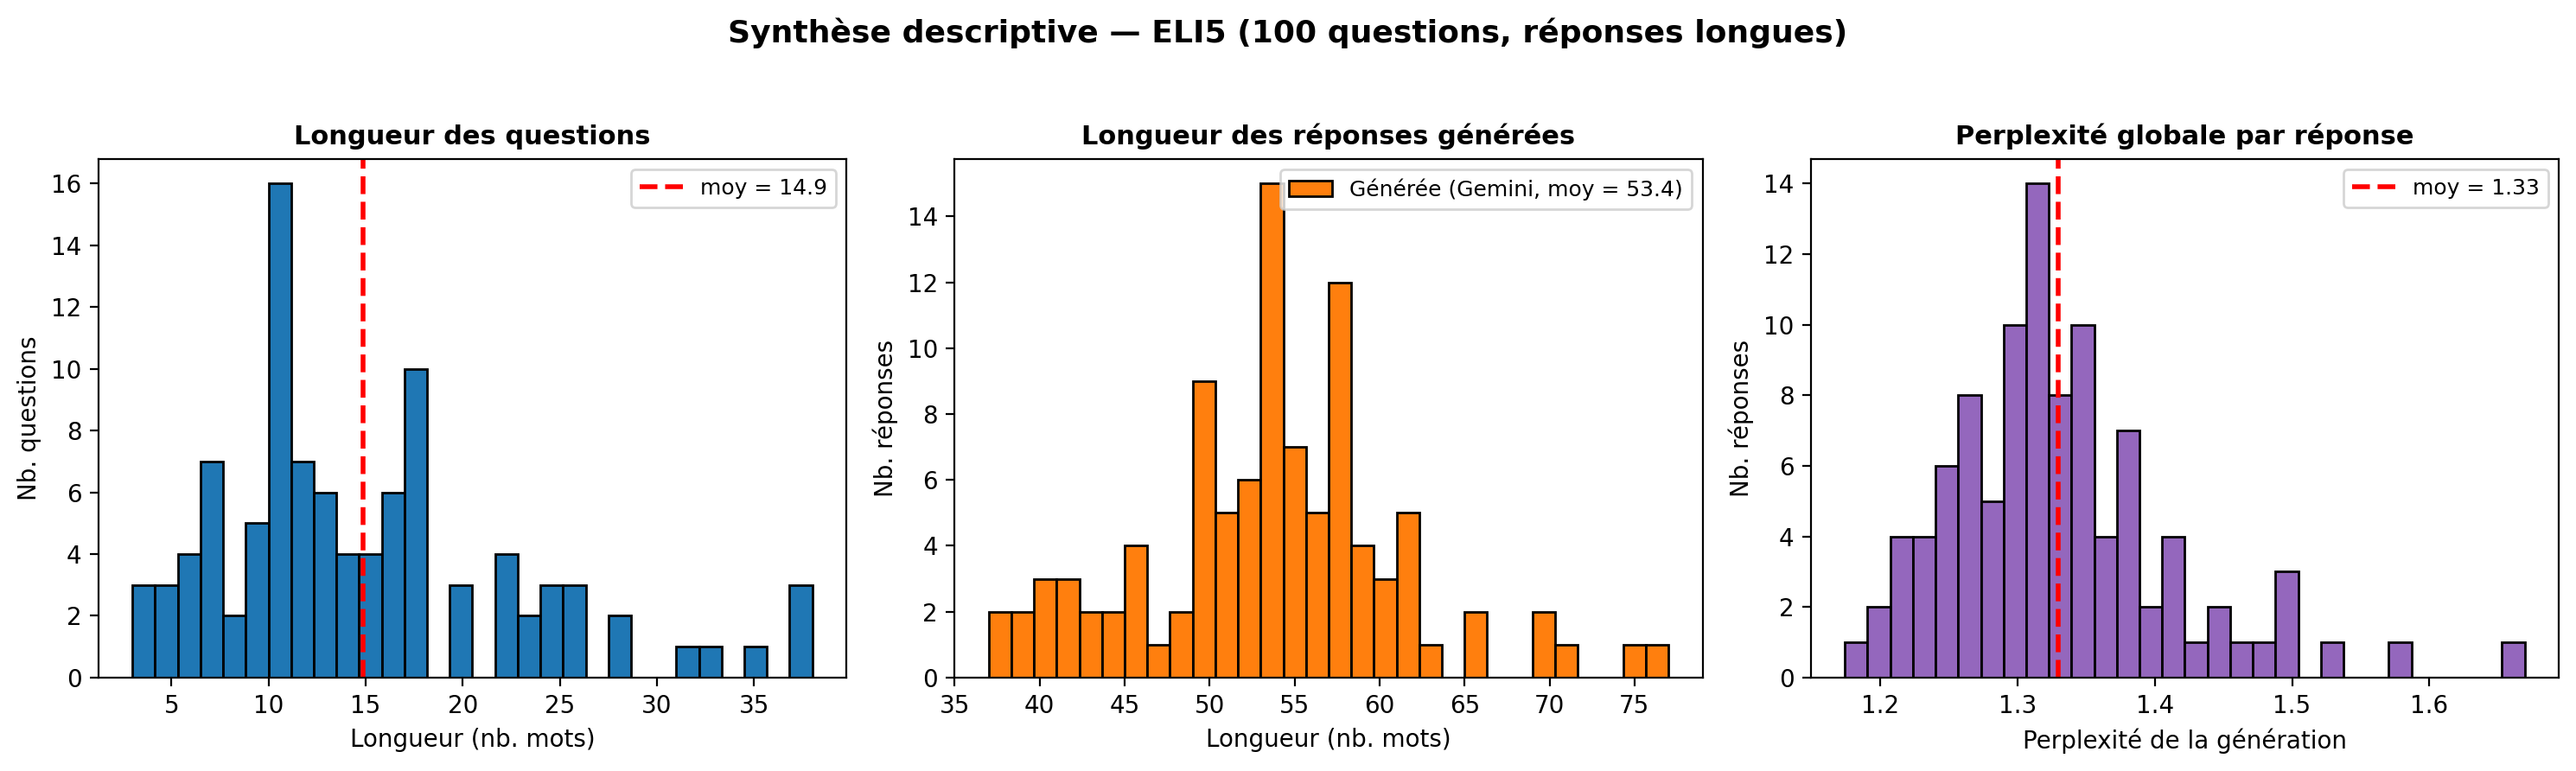
\includegraphics[width=0.95\textwidth]{stats_eli5.png}
    \caption{Synthèse descriptive d'ELI5 (100 questions).}
    \label{fig:eli5_stats}
\end{figure}

\section{Définition formelle des scores de confiance (TriviaQA)}
\label{ann:scores_definitions}

Soit $(t_1, \ldots, t_T)$ la séquence de tokens générée pour la question $x_i$, et $p_k = p(t_k|t_{<k}, x_i)$ la probabilité conditionnelle de chaque token. Les scores comparés en section~\ref{sec:confiance_verite} sont~:
\begin{align*}
P_i^{(\text{joint})} &= \prod_{k=1}^{T} p_k & \text{(probabilité jointe)}\\
P_i^{(\text{geo})} &= \left(\prod_{k=1}^{T} p_k\right)^{1/T} & \text{(moyenne géométrique)}\\
\text{Perplexity}_i &= \exp\left(-\frac{1}{T}\sum_k \log p_k\right) & \text{(perplexité)}\\
p_{\min,i} &= \min_k p_k & \text{(probabilité minimale)}
\end{align*}
Chaque score est calculé une fois sur l'ensemble de la génération et une fois en restreignant aux tokens correspondant à la réponse numérique extraite par parsing JSON. La confiance verbalisée $C^{(\text{verb})}_i$ et la confiance par jugement externe $C^{(\text{judge})}_i$ sont obtenues par les prompts décrits en annexe~\ref{ann:prompts}.

\section{Tableaux complets section TriviaQA-num}
\label{ann:tables_triviaqa}

\subsection{Distribution des scores}

\begin{figure}[H]
    \centering
    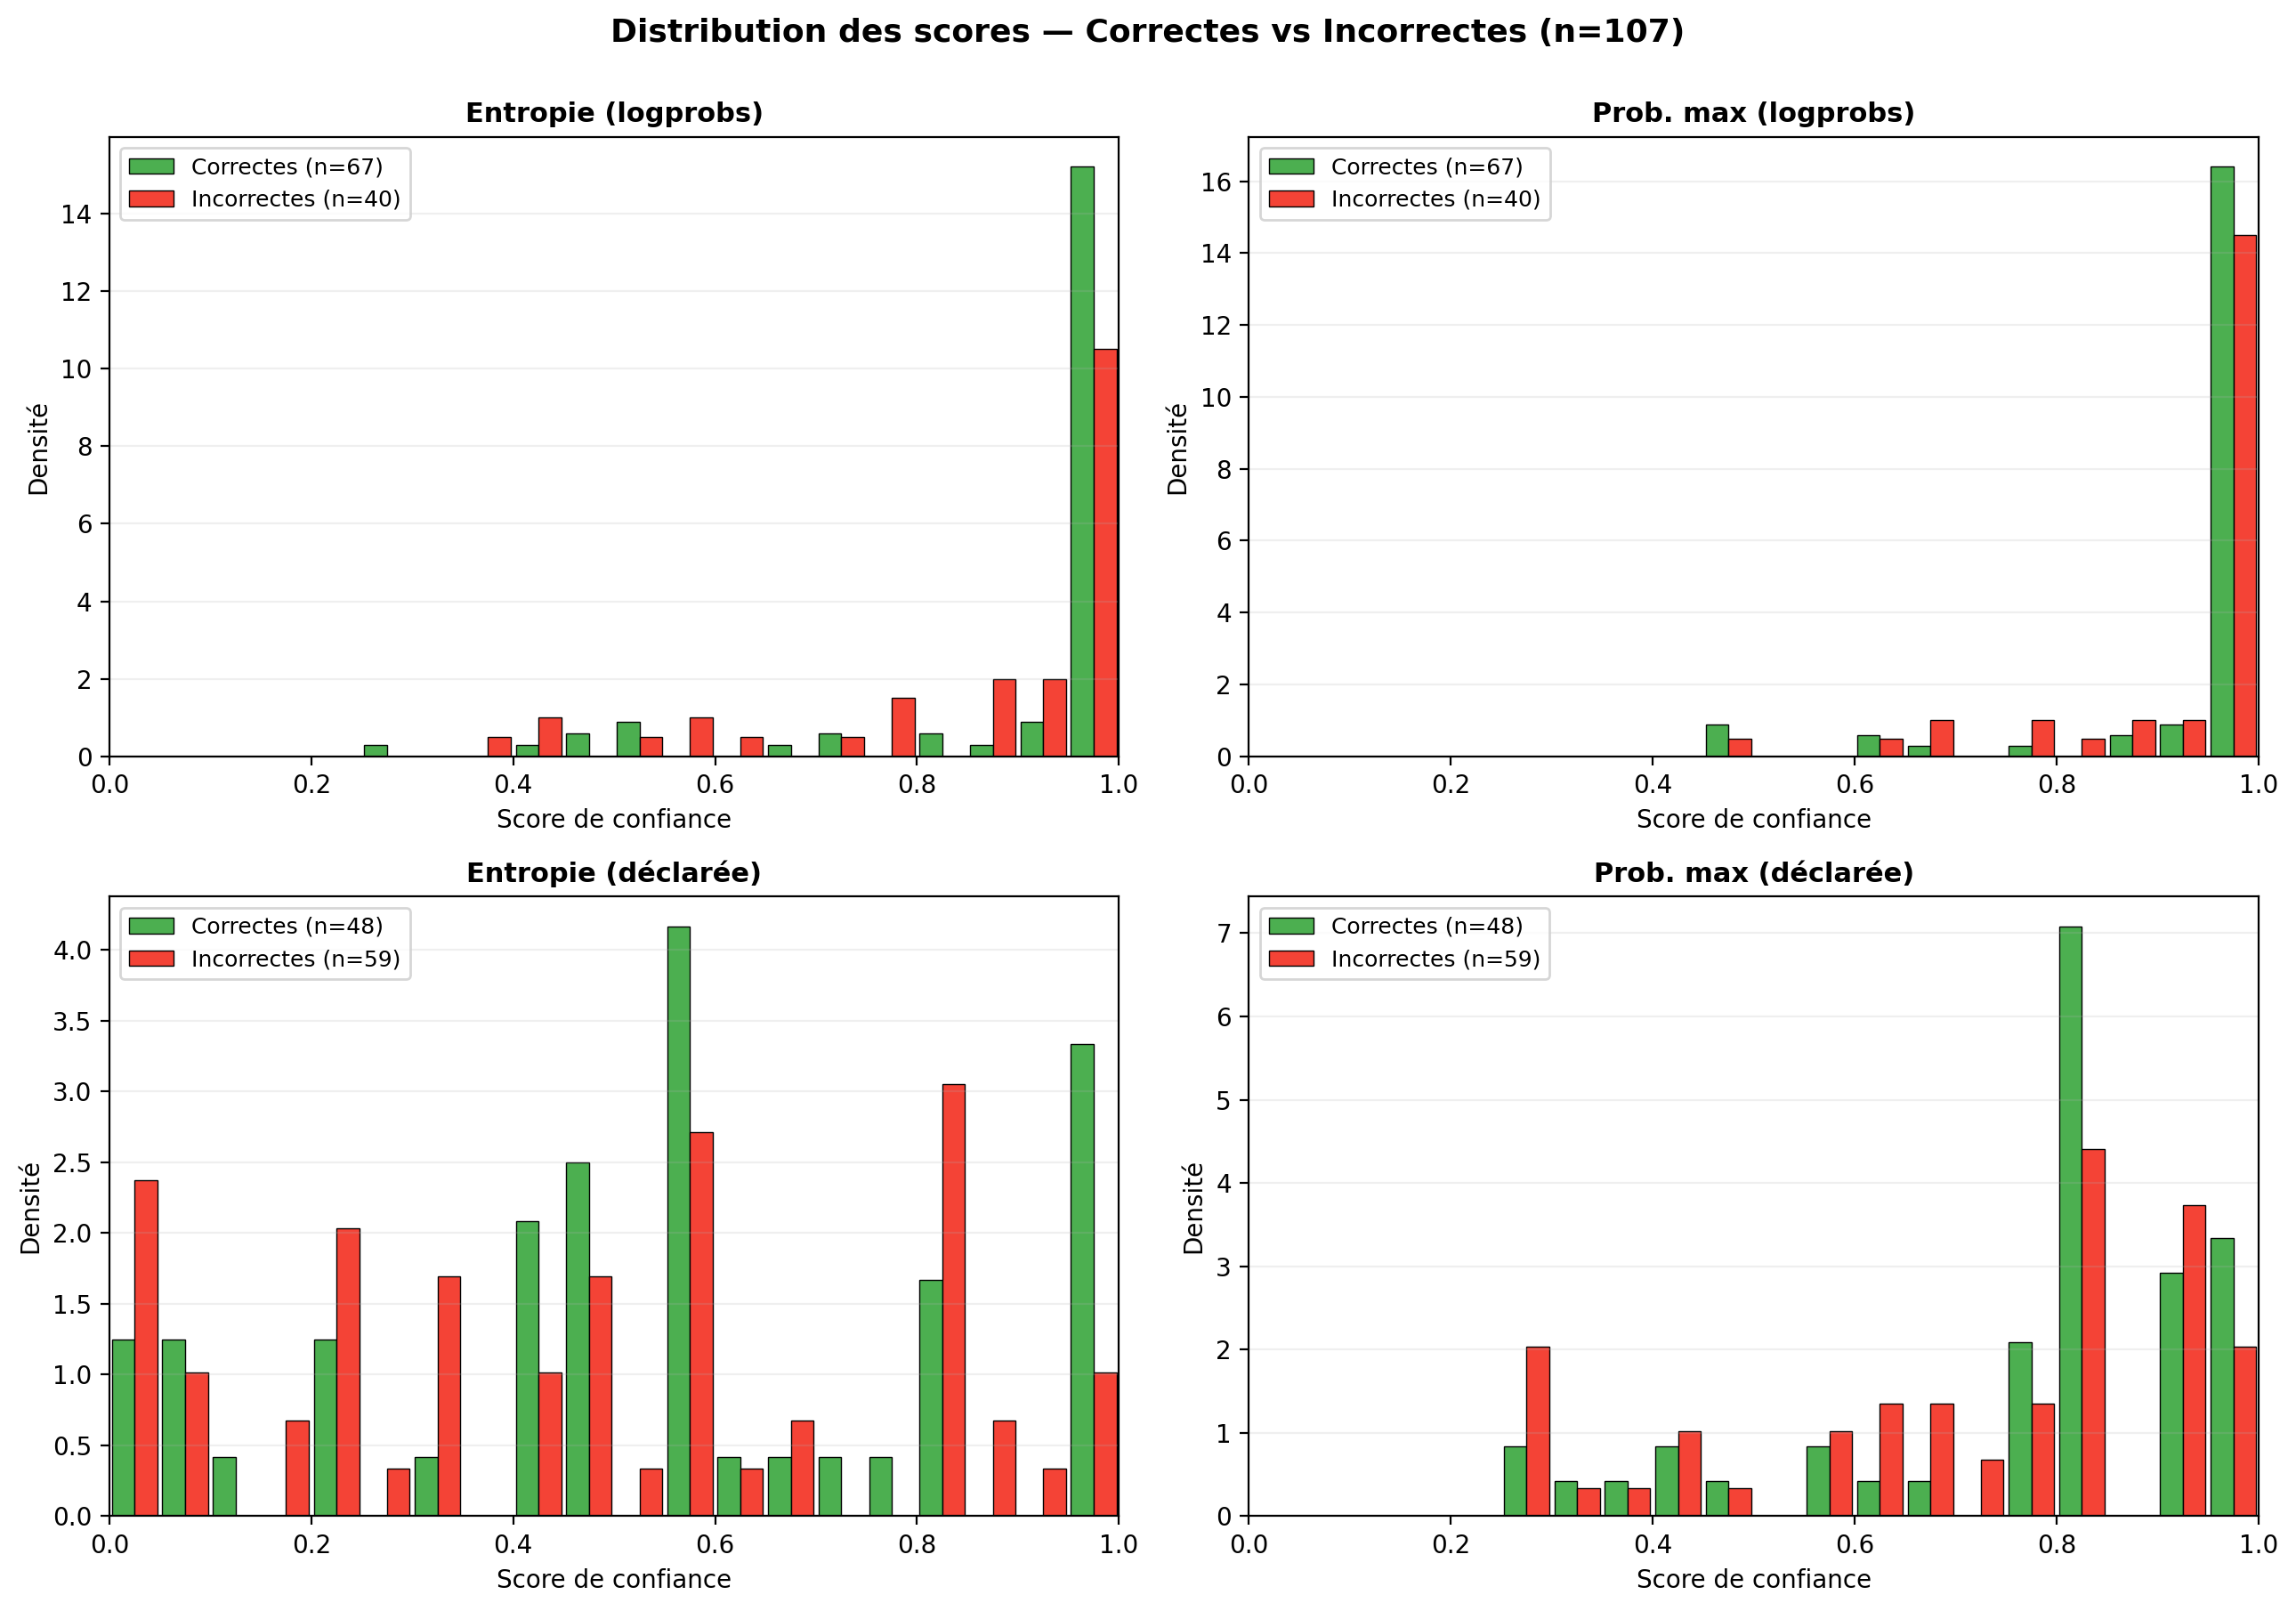
\includegraphics[width=0.95\textwidth]{fig4_confidence_distributions.png}
    \caption{Distribution des scores de confiance selon la justesse des réponses.}
    \label{fig:dist_scores}
\end{figure}

\begin{figure}[H]
    \centering
    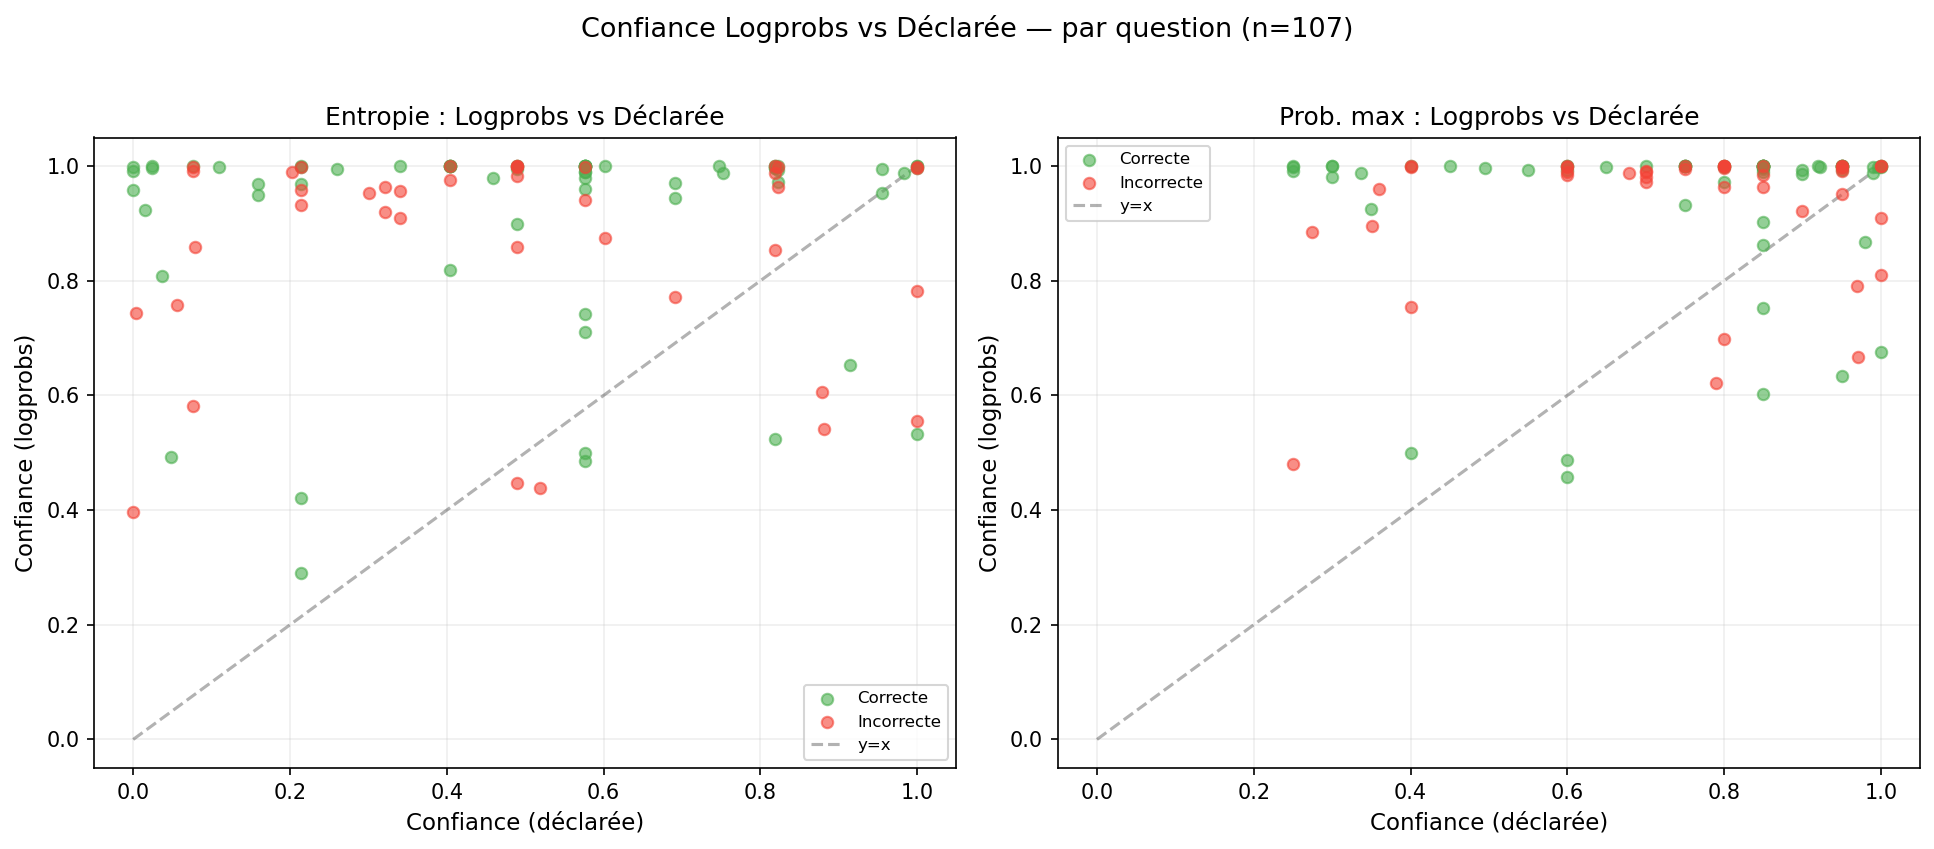
\includegraphics[width=0.85\textwidth]{fig5_logprob_vs_declared.png}
    \caption{Log-probabilités vs confiance déclarée. Les points au-dessus de la diagonale indiquent une confiance interne supérieure à la confiance verbalisée.}
    \label{fig:scatter_conf}
\end{figure}

\subsection{Tableaux numériques}

{\tiny
\begin{longtable}{p{4.0cm}rrrrl}
\caption{Résumé descriptif des différents scores de confiance} \label{tab:confidence_dispersion} \\
\toprule
Confidence score & n & Mean & Min & Max \\
\midrule
\endfirsthead
\caption[]{Résumé descriptif des différents scores de confiance} \\
\toprule
Confidence score & n & Mean & Min & Max \\
\midrule
\endhead
\midrule
\multicolumn{5}{r}{Continued on next page} \\
\midrule
\endfoot
\bottomrule
\endlastfoot
Conf verbalisée & 3395 & 0.959623 & 0.100000 & 1.000000 \\
Conf judge & 3391 & 0.908139 & 0.010000 & 1.000000 \\
Prob joint seq & 3395 & 0.973050 & 0.000001 & 1.000000 \\
Prob mean seq & 3395 & 0.986256 & 0.101102 & 1.000000 \\
Logprob sum seq & 3395 & -0.054219 & -13.531101 & 0.000013 \\
Logprob mean seq & 3395 & -0.018517 & -2.291625 & 0.000004 \\
Perplexity seq & 3395 & 1.029233 & 0.999996 & 9.890997 \\
Prob min seq & 3395 & 0.974415 & 0.041966 & 1.000004 \\
Prob joint all & 3395 & 0.643894 & 0.000000 & 0.998803 \\
Prob mean all & 3395 & 0.978124 & 0.629143 & 0.999954 \\
Logprob sum all & 3395 & -0.632608 & -16.218891 & -0.001197 \\
Logprob mean all & 3395 & -0.022516 & -0.463397 & -0.000046 \\
Perplexity all & 3395 & 1.023202 & 1.000046 & 1.589464 \\
Prob min all & 3395 & 0.664897 & 0.038462 & 0.999041 \\
\end{longtable}

}

\bigskip

{\tiny
\begin{longtable}{p{4.0cm}rrrrrrr}
\caption{Capacité de discrimination des scores de confiance mesurée par l'AUC} \label{tab:confidence_auc} \\
\toprule
Confidence score & n & Accuracy & AUC \\
\midrule
\endfirsthead
\caption[]{Capacité de discrimination des scores de confiance mesurée par l'AUC} \\
\toprule
Confidence score & n & Accuracy & AUC \\
\midrule
\endhead
\midrule
\multicolumn{4}{r}{Continued on next page} \\
\midrule
\endfoot
\bottomrule
\endlastfoot
Logprob mean seq & 3395 & 0.863623 & 0.857214 \\
Logprob sum seq & 3395 & 0.863623 & 0.856671 \\
Prob min seq & 3395 & 0.863623 & 0.849128 \\
Prob mean seq & 3395 & 0.863623 & 0.843973 \\
Prob joint seq & 3395 & 0.863623 & 0.843529 \\
Conf verbalisée & 3395 & 0.863623 & 0.719345 \\
Conf judge & 3391 & 0.864347 & 0.679321 \\
Prob mean all & 3395 & 0.863623 & 0.631333 \\
Logprob mean all & 3395 & 0.863623 & 0.631333 \\
Prob joint all & 3395 & 0.863623 & 0.628024 \\
Logprob sum all & 3395 & 0.863623 & 0.628024 \\
Prob min all & 3395 & 0.863623 & 0.599377 \\
Perplexity all & 3395 & 0.863623 & 0.368667 \\
Perplexity seq & 3395 & 0.863623 & 0.142786 \\
\end{longtable}

}

\bigskip

{\tiny
\begin{longtable}{lrr}
\caption{Indicateurs de calibration des scores probabilistes} \label{tab:confidence_calibration} \\
\toprule
Confidence score & Brier & ECE \\
\midrule
\endfirsthead
\caption[]{Indicateurs de calibration des scores probabilistes} \\
\toprule
Confidence score & Brier & ECE \\
\midrule
\endhead
\midrule
\multicolumn{3}{r}{Continued on next page} \\
\midrule
\endfoot
\bottomrule
\endlastfoot
Prob joint seq & 0.113852 & 0.113843 \\
Conf verbalisée & 0.117459 & 0.096000 \\
Prob mean seq & 0.120535 & 0.122633 \\
Conf judge & 0.124606 & 0.081828 \\
Prob mean all & 0.127775 & 0.114501 \\
Prob min all & 0.212136 & 0.223550 \\
Prob joint all & 0.215552 & 0.242211 \\
\end{longtable}

}

\clearpage

{\tiny
\begin{longtable}{p{4.0cm}p{2.5cm}rrrll}
\caption{Corrélations entre les signaux de confiance et la distance à la vérité terrain (ensemble des réponses)} \label{tab:confidence_distance_all} \\
\toprule
Confidence score & Distance & n & Pearson & Spearman & Effect \\
\midrule
\endfirsthead
\caption[]{Corrélations entre les signaux de confiance et la distance à la vérité terrain (ensemble des réponses)} \\
\toprule
Confidence score & Distance & n & Pearson & Spearman & Effect \\
\midrule
\endhead
\midrule
\multicolumn{6}{r}{Continued on next page} \\
\midrule
\endfoot
\bottomrule
\endlastfoot
Conf verbalisée & abs\_error & 3395 & -0.042457 & -0.270188 & faible à modéré \\
Conf verbalisée & log1p\_abs\_error & 3395 & -0.284130 & -0.270188 & faible à modéré \\
Conf verbalisée & log\_error & 3395 & -0.126969 & -0.264358 & faible à modéré \\
Conf verbalisée & rel\_error & 3395 & -0.044167 & -0.261465 & faible à modéré \\
Conf judge & abs\_error & 3391 & -0.015042 & -0.266805 & faible à modéré \\
Conf judge & log1p\_abs\_error & 3391 & -0.162569 & -0.266805 & faible à modéré \\
Conf judge & log\_error & 3391 & -0.111472 & -0.265185 & faible à modéré \\
Conf judge & rel\_error & 3391 & -0.017058 & -0.263898 & faible à modéré \\
Logprob mean all & abs\_error & 3395 & -0.018171 & -0.156858 & faible \\
Logprob mean all & log1p\_abs\_error & 3395 & -0.156985 & -0.156858 & faible \\
Logprob mean all & log\_error & 3395 & -0.063546 & -0.158993 & faible \\
Logprob mean all & rel\_error & 3395 & -0.021559 & -0.155558 & faible \\
Logprob sum all & abs\_error & 3395 & -0.024755 & -0.152897 & faible \\
Logprob sum all & log1p\_abs\_error & 3395 & -0.152380 & -0.152897 & faible \\
Logprob sum all & log\_error & 3395 & -0.062083 & -0.154579 & faible \\
Logprob sum all & rel\_error & 3395 & -0.028308 & -0.151168 & faible \\
Prob min all & abs\_error & 3395 & -0.011096 & -0.117806 & faible \\
Prob min all & log1p\_abs\_error & 3395 & -0.088027 & -0.117806 & faible \\
Prob min all & log\_error & 3395 & -0.031333 & -0.118992 & faible \\
Prob min all & rel\_error & 3395 & -0.014023 & -0.115786 & faible \\
Perplexity all & abs\_error & 3395 & 0.017245 & 0.156858 & faible \\
Perplexity all & log1p\_abs\_error & 3395 & 0.156418 & 0.156858 & faible \\
Perplexity all & log\_error & 3395 & 0.062005 & 0.158993 & faible \\
Perplexity all & rel\_error & 3395 & 0.020503 & 0.155558 & faible \\
Prob mean all & abs\_error & 3395 & -0.018971 & -0.156858 & faible \\
Prob mean all & log1p\_abs\_error & 3395 & -0.156938 & -0.156858 & faible \\
Prob mean all & log\_error & 3395 & -0.064649 & -0.158993 & faible \\
Prob mean all & rel\_error & 3395 & -0.022465 & -0.155558 & faible \\
Prob joint all & abs\_error & 3395 & -0.030863 & -0.152897 & faible \\
Prob joint all & log1p\_abs\_error & 3395 & -0.135008 & -0.152897 & faible \\
Prob joint all & log\_error & 3395 & -0.063948 & -0.154579 & faible \\
Prob joint all & rel\_error & 3395 & -0.035082 & -0.151168 & faible \\
Logprob mean seq & abs\_error & 3395 & -0.002167 & -0.425641 & modéré \\
Logprob mean seq & log1p\_abs\_error & 3395 & -0.230650 & -0.425641 & modéré \\
Logprob mean seq & log\_error & 3395 & -0.103590 & -0.426609 & modéré \\
Logprob mean seq & rel\_error & 3395 & -0.002963 & -0.425326 & modéré \\
Logprob sum seq & abs\_error & 3395 & -0.014186 & -0.425553 & modéré \\
Logprob sum seq & log1p\_abs\_error & 3395 & -0.192564 & -0.425553 & modéré \\
Logprob sum seq & log\_error & 3395 & -0.077316 & -0.426768 & modéré \\
Logprob sum seq & rel\_error & 3395 & -0.015566 & -0.425616 & modéré \\
Prob min seq & abs\_error & 3395 & -0.025617 & -0.414901 & modéré \\
Prob min seq & log1p\_abs\_error & 3395 & -0.277212 & -0.414901 & modéré \\
Prob min seq & log\_error & 3395 & -0.129688 & -0.415452 & modéré \\
Prob min seq & rel\_error & 3395 & -0.027940 & -0.413848 & modéré \\
Perplexity seq & abs\_error & 3395 & -0.000183 & 0.425641 & modéré \\
Perplexity seq & log1p\_abs\_error & 3395 & 0.170671 & 0.425641 & modéré \\
Perplexity seq & log\_error & 3395 & 0.070058 & 0.426609 & modéré \\
Perplexity seq & rel\_error & 3395 & 0.000278 & 0.425326 & modéré \\
Prob mean seq & abs\_error & 3395 & -0.005150 & -0.493118 & modéré \\
Prob mean seq & log1p\_abs\_error & 3395 & -0.262131 & -0.493118 & modéré \\
Prob mean seq & log\_error & 3395 & -0.123225 & -0.495540 & modéré \\
Prob mean seq & rel\_error & 3395 & -0.006231 & -0.492954 & modéré \\
Prob joint seq & abs\_error & 3395 & -0.042301 & -0.492527 & modéré \\
Prob joint seq & log1p\_abs\_error & 3395 & -0.294001 & -0.492527 & modéré \\
Prob joint seq & log\_error & 3395 & -0.141104 & -0.494483 & modéré \\
Prob joint seq & rel\_error & 3395 & -0.045566 & -0.491914 & modéré \\
\end{longtable}

}

\clearpage

{\tiny
\begin{longtable}{p{4.0cm}p{2.5cm}rrrll}
\caption{Corrélations entre les signaux de confiance et la distance à la vérité terrain (réponses incorrectes uniquement)} \label{tab:confidence_distance_wrong_only} \\
\toprule
Confidence score & Distance & n & Pearson & Spearman & Effect \\
\midrule
\endfirsthead
\caption[]{Corrélations entre les signaux de confiance et la distance à la vérité terrain (réponses incorrectes uniquement)} \\
\toprule
Confidence score & Distance & n & Pearson & Spearman & Effect \\
\midrule
\endhead
\midrule
\multicolumn{6}{r}{Continued on next page} \\
\midrule
\endfoot
\bottomrule
\endlastfoot
Conf verbalisée & abs\_error & 463 & -0.030027 & -0.131958 & faible \\
Conf verbalisée & log1p\_abs\_error & 463 & -0.119430 & -0.131958 & faible \\
Conf verbalisée & log\_error & 463 & -0.053670 & 0.142835 & faible \\
Conf verbalisée & rel\_error & 463 & -0.035792 & 0.156776 & faible \\
Conf judge & abs\_error & 460 & -0.006305 & -0.032685 & quasi nul \\
Conf judge & log1p\_abs\_error & 460 & -0.125426 & -0.032685 & quasi nul \\
Conf judge & log\_error & 460 & -0.129213 & 0.037922 & quasi nul \\
Conf judge & rel\_error & 460 & -0.012207 & 0.047376 & quasi nul \\
Logprob mean all & abs\_error & 463 & -0.005060 & -0.047283 & quasi nul \\
Logprob mean all & log1p\_abs\_error & 463 & -0.011949 & -0.047283 & quasi nul \\
Logprob mean all & log\_error & 463 & -0.003188 & -0.039990 & quasi nul \\
Logprob mean all & rel\_error & 463 & -0.012972 & -0.021579 & quasi nul \\
Logprob sum all & abs\_error & 463 & -0.016364 & -0.043605 & quasi nul \\
Logprob sum all & log1p\_abs\_error & 463 & -0.013528 & -0.043605 & quasi nul \\
Logprob sum all & log\_error & 463 & -0.004346 & -0.021224 & quasi nul \\
Logprob sum all & rel\_error & 463 & -0.024170 & -0.003246 & quasi nul \\
Prob min all & abs\_error & 463 & -0.006719 & -0.002648 & quasi nul \\
Prob min all & log1p\_abs\_error & 463 & -0.009901 & -0.002648 & quasi nul \\
Prob min all & log\_error & 463 & 0.009012 & 0.038276 & quasi nul \\
Prob min all & rel\_error & 463 & -0.016270 & 0.053115 & très faible \\
Perplexity all & abs\_error & 463 & 0.003264 & 0.047283 & quasi nul \\
Perplexity all & log1p\_abs\_error & 463 & 0.008786 & 0.047283 & quasi nul \\
Perplexity all & log\_error & 463 & 0.000089 & 0.039990 & quasi nul \\
Perplexity all & rel\_error & 463 & 0.010631 & 0.021579 & quasi nul \\
Prob mean all & abs\_error & 463 & -0.006841 & -0.047283 & quasi nul \\
Prob mean all & log1p\_abs\_error & 463 & -0.015102 & -0.047283 & quasi nul \\
Prob mean all & log\_error & 463 & -0.006134 & -0.039990 & quasi nul \\
Prob mean all & rel\_error & 463 & -0.015233 & -0.021579 & quasi nul \\
Prob joint all & abs\_error & 463 & -0.047488 & -0.043605 & quasi nul \\
Prob joint all & log1p\_abs\_error & 463 & -0.061255 & -0.043605 & quasi nul \\
Prob joint all & log\_error & 463 & -0.041647 & -0.021224 & quasi nul \\
Prob joint all & rel\_error & 463 & -0.060540 & -0.003246 & quasi nul \\
Logprob mean seq & abs\_error & 463 & 0.023010 & -0.146024 & faible \\
Logprob mean seq & log1p\_abs\_error & 463 & -0.003988 & -0.146024 & faible \\
Logprob mean seq & log\_error & 463 & -0.012803 & -0.214042 & faible à modéré \\
Logprob mean seq & rel\_error & 463 & 0.019848 & -0.192430 & faible \\
Logprob sum seq & abs\_error & 463 & 0.005245 & -0.152643 & faible \\
Logprob sum seq & log1p\_abs\_error & 463 & -0.003516 & -0.152643 & faible \\
Logprob sum seq & log\_error & 463 & -0.000056 & -0.185736 & faible \\
Logprob sum seq & rel\_error & 463 & 0.001876 & -0.165006 & faible \\
Prob min seq & abs\_error & 463 & 0.000384 & -0.132909 & faible \\
Prob min seq & log1p\_abs\_error & 463 & -0.032132 & -0.132909 & faible \\
Prob min seq & log\_error & 463 & -0.032686 & -0.158881 & faible \\
Prob min seq & rel\_error & 463 & -0.005630 & -0.138356 & faible \\
Perplexity seq & abs\_error & 463 & -0.018036 & 0.146024 & faible \\
Perplexity seq & log1p\_abs\_error & 463 & 0.000509 & 0.146024 & faible \\
Perplexity seq & log\_error & 463 & 0.001004 & 0.214042 & faible à modéré \\
Perplexity seq & rel\_error & 463 & -0.015957 & 0.192430 & faible \\
Prob mean seq & abs\_error & 463 & 0.024038 & -0.149965 & faible \\
Prob mean seq & log1p\_abs\_error & 463 & -0.010225 & -0.149965 & faible \\
Prob mean seq & log\_error & 463 & -0.023712 & -0.222229 & faible à modéré \\
Prob mean seq & rel\_error & 463 & 0.020074 & -0.198807 & faible \\
Prob joint seq & abs\_error & 463 & -0.020382 & -0.152014 & faible \\
Prob joint seq & log1p\_abs\_error & 463 & -0.051953 & -0.152014 & faible \\
Prob joint seq & log\_error & 463 & -0.044534 & -0.180300 & faible \\
Prob joint seq & rel\_error & 463 & -0.027630 & -0.158374 & faible \\
\end{longtable}

}

\section{Indicateurs et tableaux pour GSM8K (générations longues)}
\label{ann:gsm_features}

\subsection{Indicateurs construits sur les log-probabilités}

Pour chaque génération $(t_1, \ldots, t_T)$ avec $\ell_k = \log p(t_k|t_{<k},x)$ et $p_k = e^{\ell_k}$~:

\paragraph{Statistiques de niveau.} Moyennes, médianes, min/max et écart-type des suites $(\ell_k)$ et $(p_k)$.

\paragraph{Incertitude.} Entropie $H_k = -\sum_v p(v|t_{<k},x)\log p(v|t_{<k},x)$ et ses agrégats ($\overline{H}, H_{\max}, H_{\min}$).

\paragraph{Marge.} $m_k = p_k^{(1)} - p_k^{(2)}$ (différence entre les deux tokens les plus probables à la position $k$).

\paragraph{Persistance.} Longueur maximale d'une plage de tokens dont la log-probabilité est inférieure à un seuil $c$~:
\[
L_c = \max\{r : \exists j, \ell_j < c, \ldots, \ell_{j+r-1} < c\}.
\]

\paragraph{Structure temporelle.} Pour une variable $z_k$, moyennes sur les tiers $I_1, I_2, I_3$ de la génération~:
\[
\overline{z}^{(j)} = \frac{1}{|I_j|}\sum_{k \in I_j} z_k,
\]
ainsi que les différences $\overline{z}^{(3)} - \overline{z}^{(1)}$.

\paragraph{Sous-séquences.} Tous les indicateurs sont calculés séparément sur les tokens du raisonnement, les tokens de la réponse finale, et l'ensemble de la génération.

\subsection{Tableaux complets}
\label{ann:tables_gsm}

{\small
\begin{table}[htbp]
\centering
\caption{Performance des différents ensembles de variables pour la détection des erreurs.}
\label{tab:logprob_model_summary}
\begin{tabular}{lccc}
\toprule
Feature set & Nb. features & ROC-AUC & Average Precision \\
\midrule
All variables & 64 & 0.729 & 0.978 \\
All variables (without length) & 61 & 0.718 & 0.976 \\
Interpretable subset & 11 & 0.698 & 0.975 \\
Reasoning only & 21 & 0.679 & 0.972 \\
Reasoning only (without length) & 20 & 0.679 & 0.972 \\
Full-generation only & 21 & 0.669 & 0.969 \\
Final-answer only & 21 & 0.665 & 0.972 \\
Full-generation only (without length) & 20 & 0.663 & 0.968 \\
\bottomrule
\end{tabular}

\end{table}

}

\bigskip

{\small
\begin{table}[htbp]
\centering
\caption{Plus discriminantes variables univariées entre réponses correctes et incorrectes.}
\label{tab:logprob_top_univariate}
\begin{tabular}{lcccc}
\toprule
Variable & Mean correct & Mean wrong & AUC & FDR-BH \\
\midrule
Full generation: entropymean on last third & 0.077 & 0.158 & 0.681 & 0.000 \\
Reasoning: entropymean on last third & 0.083 & 0.177 & 0.681 & 0.000 \\
Reasoning: entropy max & 1.220 & 1.349 & 0.675 & 0.000 \\
Full generation: entropy max & 1.220 & 1.349 & 0.674 & 0.000 \\
Full generation: top1mean on last third & -0.045 & -0.099 & 0.670 & 0.000 \\
Reasoning: entropy std & 0.249 & 0.300 & 0.668 & 0.000 \\
Full generation: entropy std & 0.247 & 0.298 & 0.668 & 0.000 \\
Reasoning: top1mean on last third & -0.049 & -0.110 & 0.667 & 0.000 \\
Full generation: entropy mean & 0.114 & 0.165 & 0.666 & 0.000 \\
Reasoning: entropy mean & 0.116 & 0.171 & 0.665 & 0.000 \\
\bottomrule
\end{tabular}

\end{table}

}

\bigskip

{\small
\begin{table}[htbp]
\centering
\caption{Coefficients du modèle logistique construit sur le sous-ensemble interprétable de variables.}
\label{tab:logprob_top_manual_coefficients}
\begin{tabular}{lc}
\toprule
Variable & Coefficient \\
\midrule
Reasoning: margin mean & 1.526 \\
Full generation: margin mean & -1.257 \\
Reasoning: entropy last minusmean on first third & -0.473 \\
Reasoning: length & -0.459 \\
Reasoning: entropy mean & -0.294 \\
Reasoning: longest run lp below -2 & 0.294 \\
Reasoning: entropy max & -0.135 \\
Full generation: length & -0.088 \\
Reasoning: margin min & 0.060 \\
Final answer: margin mean & 0.026 \\
Reasoning: top1 min & 0.021 \\
\bottomrule
\end{tabular}

\end{table}

}

\section{Prédiction conforme sur MMLU : compléments}
\label{ann:conformal}

\subsection{Scores de non-conformité}

Soient $(p_{i,A}, p_{i,B}, p_{i,C}, p_{i,D})$ les probabilités softmax obtenues à partir des log-probabilités des quatre options pour la question $i$. On note $p_{(1)} \geq p_{(2)} \geq p_{(3)} \geq p_{(4)}$ les probabilités triées par ordre décroissant.

\paragraph{LAC.} Le score de non-conformité est $s_{\text{LAC}}(x_i, y) = 1 - p_{i,y}$. Pour un seuil $\hat{q}_\alpha$, l'ensemble est $\mathcal{C}_{\text{LAC}}(x_i) = \{y : p_{i,y} \geq 1 - \hat{q}_\alpha\}$.

\paragraph{APS.} Le score cumule les masses des options strictement plus probables, plus celle de l'option courante~:
\[
s_{\text{APS}}(x_i, y) = \sum_{j : p_{(j)} > p_{i,y}} p_{(j)} + p_{i,y}.
\]
L'ensemble s'obtient en empilant les options par probabilité décroissante jusqu'à atteindre la masse $\hat{q}_\alpha$.

\subsection{Protocole de calibration}

Sur les $107$ questions disposant des log-probabilités complètes, nous tirons aléatoirement un split calibration/test de tailles approximatives $50/57$. Le quantile empirique
\[
\hat{q}_\alpha = \text{Quantile}\Big(\{s_i\}_{i=1}^{n_{\text{cal}}};\; \tfrac{\lceil (n_{\text{cal}}+1)(1-\alpha)\rceil}{n_{\text{cal}}}\Big)
\]
est calculé sur le split calibration. Les couvertures et tailles moyennes reportées dans le tableau~\ref{tab:conformal_summary} sont mesurées sur le split test. Le faible nombre de calibration ($n_{\text{cal}} \simeq 50$) explique la variabilité importante des couvertures empiriques autour de la cible $1-\alpha$ et la légère sous-couverture occasionnelle de LAC.

\section{WEPR : compléments}
\label{ann:wepr}

\subsection{Courbes ROC et distributions de score}

\begin{figure}[H]
\centering
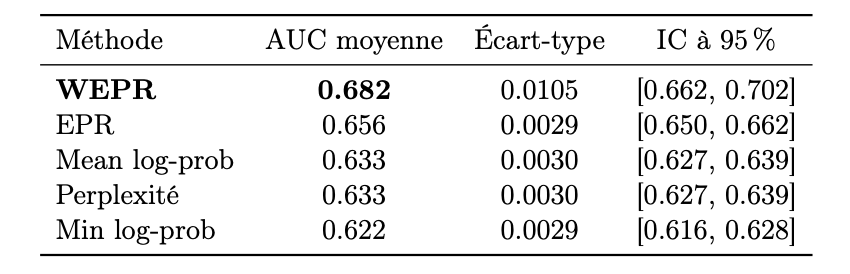
\includegraphics[width=0.75\textwidth]{roc_wepr.png}
\caption{Courbes ROC comparant WEPR aux baselines non supervisées.}
\label{fig:wepr_roc}
\end{figure}

\begin{figure}[H]
\centering
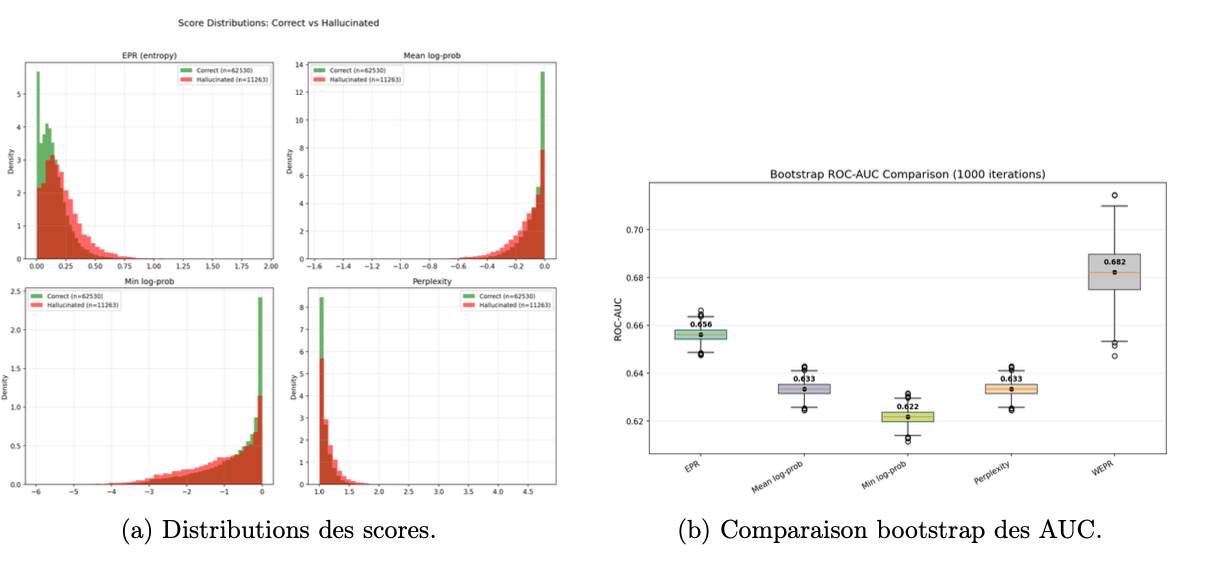
\includegraphics[width=0.75\textwidth]{score_distribution.png}
\caption{Distribution des scores WEPR pour réponses correctes et erreurs.}
\end{figure}

\subsection{Coefficients de la régression logistique et inversion de signe}
\label{ann:wepr_coefs}

Les coefficients standardisés du modèle complet sont~: $\beta_0 = +1{,}82$, $\beta_1 = +0{,}52$, $\beta_2 = -0{,}56$, $\beta_{10} = -0{,}13$, $\gamma_1 = -0{,}19$, $\gamma_{10} = -0{,}17$. L'intercept $\beta_0$ absorbe le biais de prévalence ($\log(0{,}847/0{,}153) \approx +1{,}71$)~; il chute à $+0{,}11$ en utilisant \texttt{class\_weight=balanced}, sans changer l'AUC.

L'inversion $\beta_1 > 0, \beta_2 < 0$ paraît contre-intuitive. Trois faits l'expliquent~: (i)~la corrélation entre $\overline{s}(1)$ et $\overline{s}(2)$ est de $+0{,}96$~; (ii)~les corrélations univariées avec $y$ sont \emph{toutes deux négatives} ($-0{,}19$ et $-0{,}18$)~; (iii)~en restreignant la régression à ces deux features, les deux coefficients restent négatifs.

\begin{table}[H]
\centering
\caption{Évolution de $\beta_1$ et $\beta_2$ selon les features incluses.}
\small
\begin{tabular}{lccc}
\toprule
Modèle & $\beta_1$ & $\beta_2$ & AUC \\
\midrule
Logistique sur $\overline{s}(1)$ seul & $-0{,}46$ & --- & $0{,}638$ \\
Logistique sur $\overline{s}(2)$ seul & --- & $-0{,}46$ & $0{,}636$ \\
Logistique sur $\overline{s}(1), \overline{s}(2)$ & $-0{,}37$ & $-0{,}10$ & $0{,}638$ \\
Logistique complète (20 features) & $\mathbf{+0{,}52}$ & $\mathbf{-0{,}56}$ & $0{,}681$ \\
\bottomrule
\end{tabular}
\end{table}

L'inversion n'apparaît que dans le modèle complet, en raison de la multicolinéarité avec $\overline{s}(3),\ldots,\overline{s}(10)$ qui absorbent l'essentiel du signal d'incertitude global. La régularisation Ridge (testée à $C \in \{10; 1; 0{,}1; 0{,}01\}$) ne corrige pas l'inversion mais réduit proportionnellement les amplitudes. \emph{Sur des features fortement corrélées, les signes des coefficients ne sont pas interprétables comme des effets bruts}~: il faut systématiquement confronter aux corrélations univariées et à des modèles plus simples.

\subsection{Extension non linéaire : XGBoost}
\label{ann:xgb}

Avec les mêmes 20 features et le même schéma de validation croisée, XGBoost (\texttt{n\_estimators=400}, \texttt{max\_depth=4}, \texttt{learning\_rate=0.05}) atteint AUC $= 0{,}706 \pm 0{,}004$, soit $+2{,}5$ points sur la régression logistique avec une variance entre folds réduite de moitié.

\paragraph{Importance des features.} Trois mesures convergentes (gain XGBoost en valeur absolue, permutation importance mesurée comme chute d'AUC, $|\text{SHAP}|$ moyen sur les observations)~:
\begin{itemize}[itemsep=0pt,topsep=2pt]
    \item \textbf{Gain XGBoost}~: \texttt{mean\_rank\_10} $= 54{,}7$ ($39{,}8\%$ du total), \texttt{mean\_rank\_9} $= 22{,}1$ ($16{,}1\%$). Les autres features se partagent $44{,}1\%$.
    \item \textbf{Permutation importance}~: \texttt{mean\_rank\_10} fait chuter l'AUC de $0{,}19$ point~; aucune autre feature ne dépasse $0{,}016$.
    \item \textbf{SHAP}~: $|\text{SHAP}|$ moyen de $0{,}542$ pour \texttt{mean\_rank\_10}, $0{,}136$ pour \texttt{mean\_rank\_9}, puis toutes les autres en deçà de $0{,}09$.
\end{itemize}

\paragraph{Mise en garde.} Toutes les features \texttt{mean\_rank\_k} sont fortement corrélées entre elles ($\rho > 0{,}97$ entre rangs adjacents). \texttt{mean\_rank\_7} a la plus forte corrélation univariée avec $y$ ($-0{,}26$), et non \texttt{mean\_rank\_10} ($-0{,}25$). Une régression logistique sur \texttt{mean\_rank\_10} seule atteint AUC $= 0{,}708$, supérieure à la régression complète~; mais une régression sur \texttt{mean\_rank\_7} seule produirait probablement la même AUC. \emph{Le rôle dominant de \texttt{mean\_rank\_10} dans XGBoost reflète la structure de partitionnement plutôt qu'une supériorité intrinsèque du dixième rang.}

\section{Transfert WEPR et entropie sémantique : compléments}
\label{ann:transfert}

\subsection{Protocole de transfert}

Le tableau~\ref{tab:transfer_wepr} du corps évalue la transférabilité de WEPR entre TriviaQA-WEPR et GSM8K. Le protocole est le suivant~:
\begin{itemize}[itemsep=0pt,topsep=2pt]
    \item \textbf{Modèle TriviaQA}~: WEPR entraîné sur l'intégralité de TriviaQA-WEPR ($n = 73\,793$, prévalence d'erreurs $15{,}3\%$), avec les $20$ features standard ($\overline{s}(k), m(k)$ pour $k=1,\ldots,10$).
    \item \textbf{Modèle GSM8K}~: WEPR entraîné sur les $1\,319$ générations GSM8K (prévalence d'erreurs $3{,}9\%$, soit $51$ exemples positifs), même vecteur de features calculé sur la génération complète.
    \item \textbf{Évaluation in-domain}~: CV stratifiée 5-folds sur le dataset d'entraînement.
    \item \textbf{Évaluation cross-domain}~: le modèle entraîné sur l'un est appliqué sur l'autre sans réajustement, après standardisation des features sur le dataset cible (la distribution moyenne/écart-type des $\overline{s}(k)$ diffère entre datasets).
\end{itemize}

\subsection{WEPR sur GSM8K par sous-séquence}

\begin{table}[H]
\centering
\caption{WEPR entraîné sur GSM8K — performance par sous-séquence (CV 5-folds). EPR désigne la baseline non supervisée sur la même sous-séquence.}
\small
\begin{tabular}{lccc}
\toprule
Sous-séquence & Tokens (moy.) & AUC WEPR (CV) & AUC EPR \\
\midrule
Full      & 188 & $0{,}726 \pm 0{,}149$ & $0{,}814$ \\
Reasoning & 180 & $0{,}717 \pm 0{,}156$ & $0{,}811$ \\
Answer    &   8 & $0{,}571 \pm 0{,}080$ & $0{,}640$ \\
\bottomrule
\end{tabular}
\end{table}

L'écart entre \emph{reasoning} et \emph{answer} confirme que le signal d'erreur réside dans le raisonnement, pas dans la conclusion. Sur GSM8K, EPR à elle seule atteint $0{,}81$~: la pondération apprise apporte peu sur ce dataset très déséquilibré, et la variance de WEPR ($0{,}15$) reflète l'instabilité due aux 51 erreurs seulement.

\subsection{Sous-ensemble aligné pour la table croisée}

La table croisée scores~$\times$~datasets (section~\ref{sec:cross_table}, figure~\ref{fig:cross_heatmap}) repose, pour les colonnes GSM8K, sur un sous-ensemble de $300$ questions tiré aléatoirement du dataset complet. Ce sous-ensemble permet d'aligner les coûts de calcul (génération de $K=5$ réponses pour l'entropie sémantique, calculs WEPR) et d'avoir une base commune avec TriviaQA-num. Sur ce sous-ensemble, les chiffres rapportés en section~\ref{sec:transfert_wepr} (WEPR-GSM8K $0{,}922$~; perplexité $0{,}804$) ne sont pas comparables à ceux de la CV intégrale (WEPR $0{,}726$ sur $n=1\,319$)~: l'écart vient à la fois du sous-échantillonnage et de la prévalence d'erreurs dans le tirage.

\subsection{Entropie sémantique : définition formelle et clustering}

Pour une question $x$ et $K$ générations $\{r_1, \ldots, r_K\}$ avec log-probabilité moyenne $\overline{\ell}_k$, on partitionne les réponses en clusters d'équivalence sémantique $\mathcal{C}_1, \ldots, \mathcal{C}_M$. La probabilité du cluster $c$ est définie par marginalisation softmax sur les log-probabilités~:
\[
P(c) = \frac{\sum_{k \in \mathcal{C}_c} \exp(\overline{\ell}_k)}{\sum_{k=1}^{K} \exp(\overline{\ell}_k)},
\qquad
\mathrm{SE} = -\sum_{c=1}^{M} P(c) \log P(c).
\]
Lorsque toutes les réponses tombent dans le même cluster, $M = 1$ et $\mathrm{SE} = 0$ par convention.

\paragraph{Clustering pour TriviaQA-num.} Les réponses étant numériques, l'équivalence sémantique est définie par identité numérique au seuil près après parsing JSON (deux réponses dont les valeurs flottantes coïncident à $10^{-6}$ relatif). Lorsque le parsing échoue, on tombe sur un \emph{fallback} NLI en demandant à un second LLM (Gemini~2.5~Flash) si deux textes désignent la même quantité numérique. Le prompt du juge NLI est reproduit en annexe~\ref{ann:prompts}.

La distribution empirique du nombre de clusters obtenus pour les $K=5$ générations est très concentrée sur la valeur $1$ (toutes les générations tombent dans le même cluster), comme le montre le tableau ci-dessous.

\begin{table}[H]
\centering
\caption{Distribution du nombre de clusters parmi les $K=5$ réponses générées (TriviaQA-num, $T=1{,}0$, $n=2\,574$).}
\small
\begin{tabular}{cc}
\toprule
Nombre de clusters & Proportion (\%) \\
\midrule
1 & $94{,}8$ \\
2 & $4{,}0$ \\
3 & $0{,}7$ \\
4 & $0{,}2$ \\
5 & $0{,}3$ \\
\bottomrule
\end{tabular}
\end{table}

\section{Prompts utilisés}
\label{ann:prompts}

Tous les prompts sont rédigés en anglais (questions de TriviaQA, GSM8K et MMLU en anglais, meilleures performances des LLMs dans cette langue). Les sorties sont demandées au format JSON ou en lettre unique pour garantir la stabilité du parsing automatique.

\subsection{TriviaQA-numérique : génération et confiance verbalisée}

\begin{verbatim}
You must answer in STRICT JSON with exactly two keys: "answer" and "confidence".

Rules:
- Return ONLY the JSON object. No extra text, no markdown, no explanation.
- "answer": a number in decimal notation (examples: 1945, 3.14, -12.5).
  No commas. No units. No text.
- "confidence": a float between 0 and 1 (inclusive). This number must be
  the confidence you have in the answer. If you respond 0.7 then 7 times
  out of 10 you are correct. Be careful, you must not overstate your
  confidence. It must be a JSON number, not a string.

Question:
{q}
\end{verbatim}

\subsection{TriviaQA-numérique : jugement externe (LLM-as-a-judge)}

\begin{verbatim}
You are an assistant that evaluates the correctness of a model's answer
to a question.

Return a single JSON object with exactly one key: "judge_confidence".

- "judge_confidence" must be a JSON number in [0, 1].
- Return ONLY the JSON object. No markdown, no extra text.

The judge confidence must be the probability that the model's answer
is correct, calibrated as best as possible. If the model's answer is
very likely correct, return a value close to 1. If it's likely
incorrect, return a value close to 0.

Question:
{question}

Model answer (numeric text):
{model_answer_text}
\end{verbatim}

\subsection{TriviaQA-WEPR : génération de la réponse libre}

Pour la constitution du dataset WEPR ($73\,793$ questions), nous utilisons un prompt plus léger qui sollicite une réponse textuelle d'une seule phrase, afin de couvrir l'intégralité du benchmark TriviaQA (et non plus uniquement les réponses numériques).

\begin{verbatim}
Answer the following question in exactly ONE short sentence.
Your sentence must contain the answer.
Do not add any preamble, explanation, or follow-up.

Question: {question}
Answer:
\end{verbatim}

\subsection{TriviaQA-WEPR : juge de factualité (annotation $Y$)}

L'étiquette d'erreur $Y \in \{0, 1\}$ utilisée pour l'apprentissage de WEPR est produite par un second LLM (Gemini~2.0~Flash) confronté aux réponses de référence du dataset original. Le juge traite les questions par lots et retourne un vecteur booléen.

\begin{verbatim}
You are a strict factuality judge for trivia questions.

RULES:
- An answer is CORRECT (true) ONLY if it explicitly contains or directly
  matches one of the ACCEPTED ANSWERS listed below.
- Do NOT use your own knowledge. If the LLM answer gives a name, date,
  or fact that is NOT in the accepted answers list, it is INCORRECT,
  even if you know it to be factually related or equivalent.
- Minor spelling variations (e.g. capitalization, punctuation) are OK.
- Synonyms, aliases, or related facts NOT in the accepted list => false.

Return ONLY a JSON object in this exact format:
{"judgments": [true, false, true, ...]}
The array MUST have exactly N elements, in the same order.
No explanations, no markdown fences, just the JSON.

--- Item 1 ---
Question: {question}
Accepted answers: {gt1 | gt2 | ... | gt8}
LLM answer: {full_answer}
...
\end{verbatim}

\subsection{GSM8K : raisonnement \emph{chain-of-thought} et réponse finale}

Pour produire les générations longues analysées en section~\ref{sec:generations_longues}, nous demandons un raisonnement détaillé suivi d'une réponse au format JSON sur la dernière ligne. Cette structure permet à la fois d'extraire la réponse pour la métrique d'exactitude et de séparer les sous-séquences \emph{raisonnement} et \emph{réponse finale} pour le calcul des features.

\begin{verbatim}
You are a careful math problem solver.

Solve the following grade-school math problem. First, work through the
problem step by step in clear English. Then, on the LAST line, output a
JSON object with the final numeric answer in the form:

{"answer": <number>}

Rules:
- The reasoning must precede the JSON. Use plain English, no markdown.
- The final line must be ONLY the JSON object — no fences, no extra text.
- "answer" must be a number in decimal notation (no commas, no units, no text).

Question:
{q}
\end{verbatim}

\subsection{MMLU : choix forcé pour extraction des log-probabilités}

Pour exploiter les log-probabilités sur les quatre options \{A, B, C, D\} (section~\ref{sec:qcm}), la sortie est contrainte à un unique caractère ASCII parmi $\{A, B, C, D\}$. Cette contrainte garantit que la première position de génération porte directement la distribution sur les quatre options et permet le calcul exact du softmax utilisé pour LAC et APS.

\begin{verbatim}
You must answer with EXACTLY ONE SINGLE LETTER among "A", "B", "C", "D".
Only ASCII uppercase letters are allowed (Unicode code points: U+0041,
U+0042, U+0043, U+0044).
No other token is acceptable: no spaces, no newlines, no punctuation,
no explanations.

Question:
{q}

A) {choice_A}
B) {choice_B}
C) {choice_C}
D) {choice_D}
\end{verbatim}

\subsection{ELI5 : génération longue}

Pour ELI5 (section~\ref{sec:transverse}), aucune contrainte JSON n'est imposée puisque la réponse n'est pas évaluable automatiquement. Le prompt demande une explication courte mais en langage naturel libre.

\begin{verbatim}
Explain the following like I'm 5 years old.
Use simple words, short sentences, and everyday analogies.
Keep your explanation to 3-5 sentences maximum.

Question: {question}

Explanation:
\end{verbatim}

\subsection{Entropie sémantique : juge NLI (clustering)}

Lorsque le clustering par identité numérique échoue (réponses non parsables, formats hétérogènes), le clustering est complété par un juge NLI qui décide si deux réponses désignent la même valeur numérique. Le juge traite les paires par lots.

\begin{verbatim}
You are a semantic equivalence judge for short factual answers.

For each pair below, decide if Answer A and Answer B convey the SAME
numeric value (after parsing).
Two answers are equivalent if they refer to the same number, allowing
minor formatting differences (1,000 vs 1000) but NOT different values.
If the values differ, even by 1, they are NOT equivalent.

Return ONLY a JSON object in this exact format:
{"equivalences": [true, false, true, ...]}
The array MUST have exactly N elements, in the same order.
No explanations, no markdown, just the JSON.

--- Pair 1 ---
Question: {q}
Answer A: {a}
Answer B: {b}
...
\end{verbatim}

% ========================================
% BIBLIOGRAPHIE
% ========================================


\begin{thebibliography}{99}

\bibitem[Xiong et al.(2024)]{xiong2024}
Xiong, M., Hu, Z., Lu, X., Li, Y., Fu, J., He, J., Hooi, B. (2024).
Can LLMs Express Their Uncertainty? An Empirical Evaluation of
Confidence Elicitation in LLMs.
\textit{ICLR 2024}.

\bibitem[Manakul et al.(2023)]{manakul2023selfcheckgpt}
Manakul, P., Liusie, A., Gales, M.~J.~F. (2023).
SelfCheckGPT: Zero-Resource Black-Box Hallucination Detection for
Generative Large Language Models.
\textit{EMNLP 2023}, arXiv:2303.08896.

\bibitem[Kuhn et al.(2023)]{kuhn2023semantic}
Kuhn, L., Gal, Y., Farquhar, S. (2023).
Semantic Uncertainty: Linguistic Invariances for Uncertainty
Estimation in Natural Language Generation.
\textit{ICLR 2023}.

\bibitem[Ye et al.(2024)]{ye2024benchmarking}
Ye, F., Yang, M., Pang, J., Wang, L., Wong, D.~F., Yilmaz, E.,
Shi, S., Tu, Z. (2024).
Benchmarking LLMs via Uncertainty Quantification.
\textit{NeurIPS 2024}.

\bibitem[Moslonka et al.(2026)]{moslonka2026}
Moslonka, C., Randrianarivo, H., Garnier, A., Malherbe, E. (2026).
Learned Hallucination Detection in Black-Box LLMs using Token-level
Entropy Production Rate.
\textit{arXiv:2509.04492v2}.

\bibitem[Brown et al.(2020)]{brown2020}
Brown, T.~B., et al. (2020).
Language Models are Few-Shot Learners.
\textit{NeurIPS 2020}.

\bibitem[Angelopoulos \& Bates(2023)]{angelopoulos2023}
Angelopoulos, A.~N., Bates, S. (2023).
Conformal Prediction: A Gentle Introduction.
\textit{Foundations and Trends in Machine Learning}, 16(4), 494--591.

\bibitem[Cobbe et al.(2021)]{cobbe2021gsm8k}
Cobbe, K., Kosaraju, V., Bavarian, M., et al. (2021).
Training Verifiers to Solve Math Word Problems.
\textit{arXiv:2110.14168}.

\bibitem[Hendrycks et al.(2021)]{hendrycks2021mmlu}
Hendrycks, D., Burns, C., Basart, S., et al. (2021).
Measuring Massive Multitask Language Understanding.
\textit{ICLR 2021}.

\bibitem[Joshi et al.(2017)]{joshi2017triviaqa}
Joshi, M., Choi, E., Weld, D.~S., Zettlemoyer, L. (2017).
TriviaQA: A Large Scale Distantly Supervised Challenge Dataset for
Reading Comprehension.
\textit{ACL 2017}.

\bibitem[Fan et al.(2019)]{fan2019eli5}
Fan, A., Jernite, Y., Perez, E., Grangier, D., Weston, J., Auli, M.
(2019).
ELI5: Long Form Question Answering.
\textit{ACL 2019}.

\end{thebibliography}

\end{document}
